\section{Evaluación aplicaciones nativa y multiplataforma}

A continuación se detalla la evaluación de los prototipos 3 y 4 ya expuestos en la Sección 3.2, los cuales poseen las mismas funcionalidades pero desarrollados con distintas herramientas, el primero utilizando el IDE Android Studio para desarrollar con el SDK nativo de android (desde ahora Droid) y el segundo prototipo utilizando el IDE VisualStudio Community en un proyecto Xamarin.Forms (desde ahora Xamarin). Ambos prototipos fueron modificados para realizar la siguiente evaluación que consta de 1,000 muestras y su almacenamiento en la memoria interna para la cantidad de motores y flexores del hardware disponible. Las pruebas fueron realizadas en el dispositivo Samsung Galaxy S5 mini y Nexus 5 ya señalados en el Capítulo 1. Para el análisis de latencia de los motores, se considerando su tiempo de activación y desactivación con una precisión de nanosegundos ($ns$), transformando los resultados a microsegundos ($\mu s$).  Por tanto el umbral límite de 60 milisegundos ($ms$) es equivalente a 60,000 $\mu s$ ó 60,000,000 $ns$ .

\subsection{Prototipo 3 : Droid - Galaxy}

\subsubsection{Motores}

Se realizaron pruebas desde uno a cinco motores , el resumen de los resultados para las pruebas de activación de los motores se encuentra en la Tabla \ref{table:motor-droid-galaxy}. La Figura \ref{fig:droid-galaxy-hist-motors}, muestra los histogramas de las latencias obtenidas al mandar los mensajes de activación y desactivación, siendo la gráfica para dos motores el único con una asimetría (Skewness) negativa, lo que indica que la cola de la distribución de los datos está orientada a la izquierda, por tanto la media de la distribución se encuentra desplazada a la derecha. Para las demás pruebas realizadas se obtuvieron asimetrías positivas, lo que indica que la cola de la distribución se encuentra a la derecha, por tanto su media se encuentra desplazada a la izquierda. Esto se ve reflejado en los gráficos de cajas de la Figura \ref{fig:droid-galaxy-boxplot-motors}. Las gráficas de Q-Q (quantile-quantile) mostradas en la Figura \ref{fig:droid-galaxy-QQ-motors}, demuestran que la curva no sigue estrictamente una distribución normal, pero los gráfico Q-Q de la misma figura, para para dos, cuatro y cinco motores muestra resultados cercanos a la normal exceptuando los valores atípicos, los cuales pueden ser apreciados también en sus respectivas gráficas de cajas. Finalmente la Curtosis (Kurtosis) de todas las pruebas fue positiva, lo que indica que las colas de estas distribuciones son más pesadas que la de una distribución normal, es decir, en comparación a ella concentran mayor cantidad de datos en las colas.

% {START} RESUME TABLE ---------------------------------
%\caption[Resumen resultado pruebas motor Droid-Galaxy]{Resumen resultado pruebas motor Droid-Galaxy \\ Fuente: Elaboración propia (2018)}
%\label{table:motor-droid-galaxy} 

% Table created by stargazer v.5.2.2 by Marek Hlavac, Harvard University. E-mail: hlavac at fas.harvard.edu
% Date and time: Tue, Jul 03, 2018 - 19:28:30
% Requires LaTeX packages: dcolumn 
\begin{table}[!htbp] \centering 
\caption[Resumen resultado pruebas motor Droid-Galaxy]{Resumen resultado pruebas motor Droid-Galaxy  en $\mu s$\\ Fuente: Elaboración propia (2018)}
\label{table:motor-droid-galaxy}
\begin{tabular}{@{\extracolsep{5pt}} D{.}{.}{-3} D{.}{.}{-3} D{.}{.}{-3} D{.}{.}{-3} D{.}{.}{-3} D{.}{.}{-3} D{.}{.}{-3} D{.}{.}{-3} } 
\\[-1.8ex]\hline 
\hline \\[-1.8ex] 
\multicolumn{1}{c}{Motors} & \multicolumn{1}{c}{Mean} & \multicolumn{1}{c}{Median} & \multicolumn{1}{c}{Min} & \multicolumn{1}{c}{Max} & \multicolumn{1}{c}{Std. Dev.} & \multicolumn{1}{c}{Skewness} & \multicolumn{1}{c}{Kurtosis} \\ 
\hline \\[-1.8ex] 
1 & 245.345 & 170.156 & 135.469 & 681.354 & 141.369 & 1.336 & 3.376 \\ 
2 & 263.026 & 272.031 & 192.084 & 357.083 & 36.334 & -0.114 & 2.965 \\ 
3 & 570.168 & 375.026 & 313.802 & 1,576.875 & 337.726 & 1.257 & 2.911 \\ 
4 & 418.957 & 424.843 & 304.688 & 668.750 & 61.357 & 0.417 & 4.613 \\ 
5 & 484.390 & 497.240 & 353.073 & 724.479 & 78.401 & 0.221 & 3.303 \\ 
\hline \\[-1.8ex] 
\end{tabular} 
\end{table} 
% {END} RESUME TABLE ---------------------------------


\begin{figure}
 \begin{center} 
   	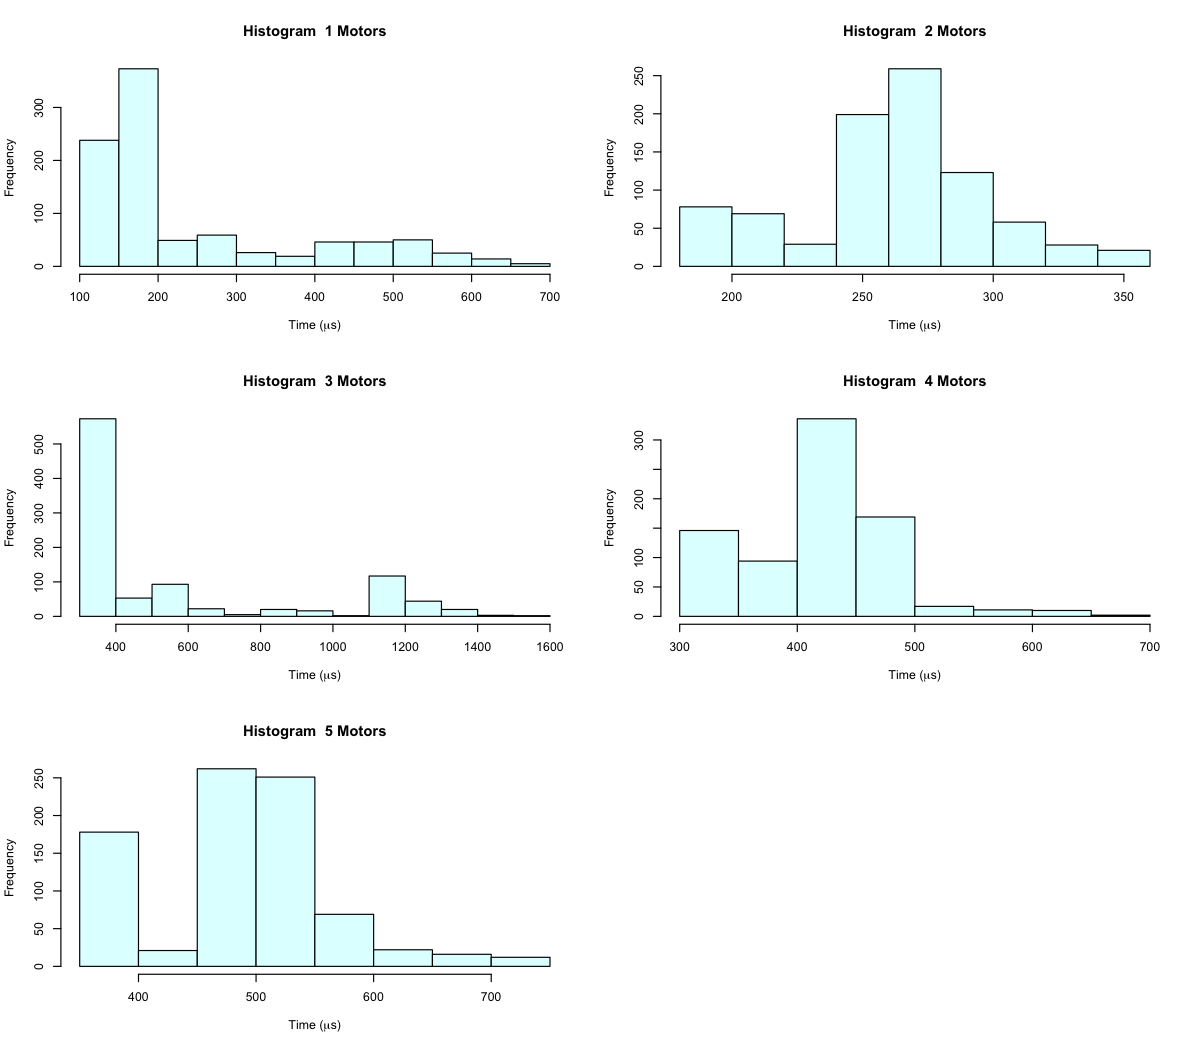
\includegraphics[width=1.0\textwidth]{evaluation/graphics/Droid/Galaxy/HistMotorsDroidGalaxy.png} 
    \caption[Histogramas de motores Droid-Galaxy]{Histogramas de motores  Droid-Galaxy\\Fuente: elaboración propia (2018)} 
    \label{fig:droid-galaxy-hist-motors}
  \end{center}
\end{figure}

\begin{figure}[H]
  \begin{center} 
   	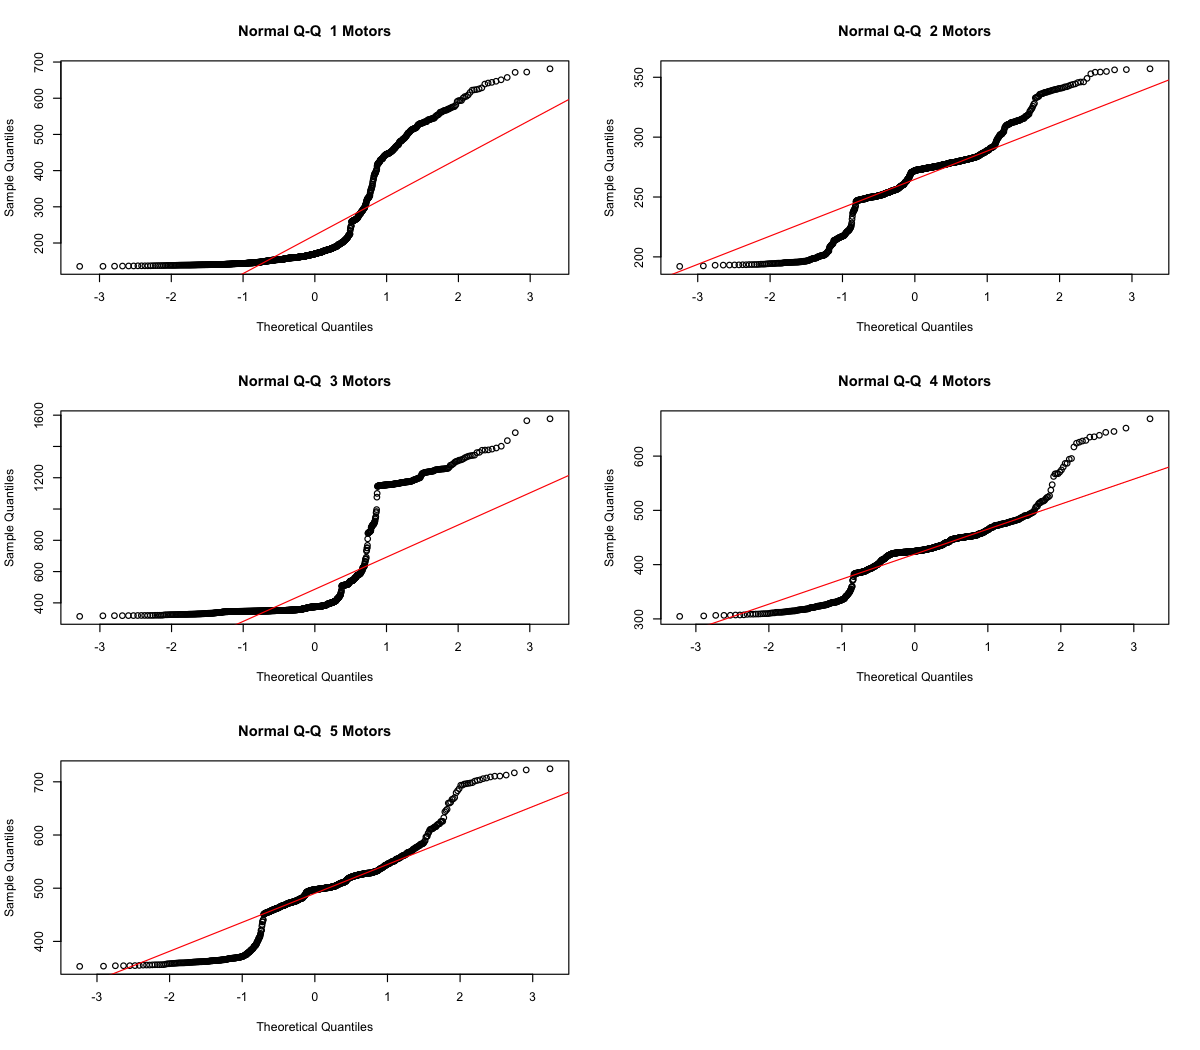
\includegraphics[width=1.0\textwidth]{evaluation/graphics/Droid/Galaxy/NormalQQMotorsDroidGalaxy.png} 
    \caption[Gráfico QQ de motores Droid-Galaxy]{Gráficos QQ de motores Droid-Galaxy\\Fuente: elaboración propia (2018)} 
    \label{fig:droid-galaxy-QQ-motors}
  \end{center}
\end{figure}

\begin{figure}[H]
  \begin{center} 
   	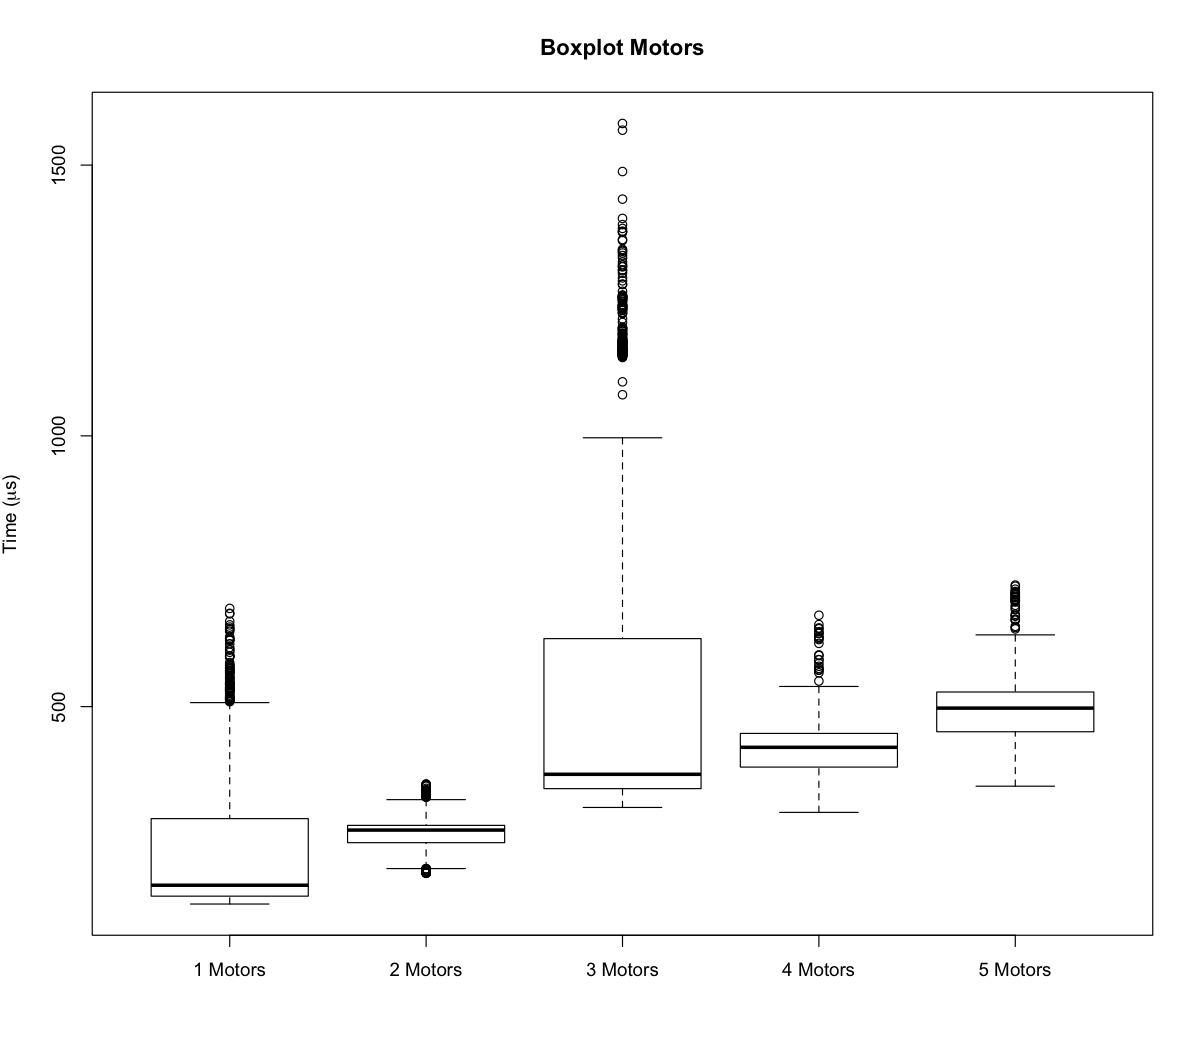
\includegraphics[width=0.8\textwidth]{evaluation/graphics/Droid/Galaxy/BoxplotMotorsDroidGalaxy.png} 
    \caption[Gráficos de cajas de motores Droid-Galaxy]{Gráficos de cajas de motores Droid-Galaxy\\Fuente: elaboración propia (2018)} 
    \label{fig:droid-galaxy-boxplot-motors}
  \end{center}
\end{figure}



\subsubsection{Flexores}
En el caso de los flexores, se realizó solamente una prueba para la obtención de datos desde la placa Arduino, con el único flexor físico disponible. Se utilizó una API de bajo nivel en Java desarrollada, en base a la C\# de bajo nivel. El resumen de los resultados de la prueba se muestra en la Tabla \ref{table:flexor-droid-galaxy}. De la tabla se puede observar que la muestra presenta una asimetría positiva, lo que implica que la cola de la distribución se encuentra a la derecha, por tanto, la media se encuentra desplazada hacia la izquierda, su Curtosis al ser positiva indica que posee mayor concentración de datos en las colas que una distribución normal. Esto puede apreciarse en el histograma de la Figura \ref{fig:droid-galaxy-hist-flexors} en conjunto con el diagrama de cajas de la Figura \ref{fig:droid-galaxy-boxplot-flexors}. En el gráfico Q-Q de la Figura \ref{fig:droid-galaxy-QQ-flexors}, se puede apreciar que la curva no sigue una distribución normal de manera estricta, sino que presenta acercamientos a ella, en forma sinusoidal.

% {START} RESUME TABLE ---------------------------------
%\extracolsep{-11pt}
%\caption[Resumen resultado pruebas flexor Droid-Galaxy]{Resumen resultado pruebas flexor Droid-Galaxy \\ Fuente: Elaboración propia (2018)}
%\label{table:flexor-droid-galaxy}

% Table created by stargazer v.5.2.2 by Marek Hlavac, Harvard University. E-mail: hlavac at fas.harvard.edu
% Date and time: Tue, Jul 03, 2018 - 19:48:03
% Requires LaTeX packages: dcolumn 
\begin{table}[!htbp] \centering 
\caption[Resumen resultado pruebas flexor Droid-Galaxy]{Resumen resultado pruebas flexor Droid-Galaxy en $\mu s$\\ Fuente: Elaboración propia (2018)}
\label{table:flexor-droid-galaxy}
\begin{tabular}{@{\extracolsep{-11pt}} D{.}{.}{-3} D{.}{.}{-3} D{.}{.}{-3} D{.}{.}{-3} D{.}{.}{-3} D{.}{.}{-3} D{.}{.}{-3} D{.}{.}{-3} } 
\\[-1.8ex]\hline 
\hline \\[-1.8ex] 
\multicolumn{1}{c}{Motors} & \multicolumn{1}{c}{Mean} & \multicolumn{1}{c}{Median} & \multicolumn{1}{c}{Min} & \multicolumn{1}{c}{Max} & \multicolumn{1}{c}{Std. Dev.} & \multicolumn{1}{c}{Skewness} & \multicolumn{1}{c}{Kurtosis} \\ 
\hline \\[-1.8ex] 
1 & 121,879.900 & 108,551.400 & 34,473.860 & 252,435.200 & 38,318.940 & 0.658 & 2.637 \\ 
\hline \\[-1.8ex] 
\end{tabular} 
\end{table} 
% {END} RESUME TABLE ---------------------------------

\begin{figure}
 \begin{center} 
   	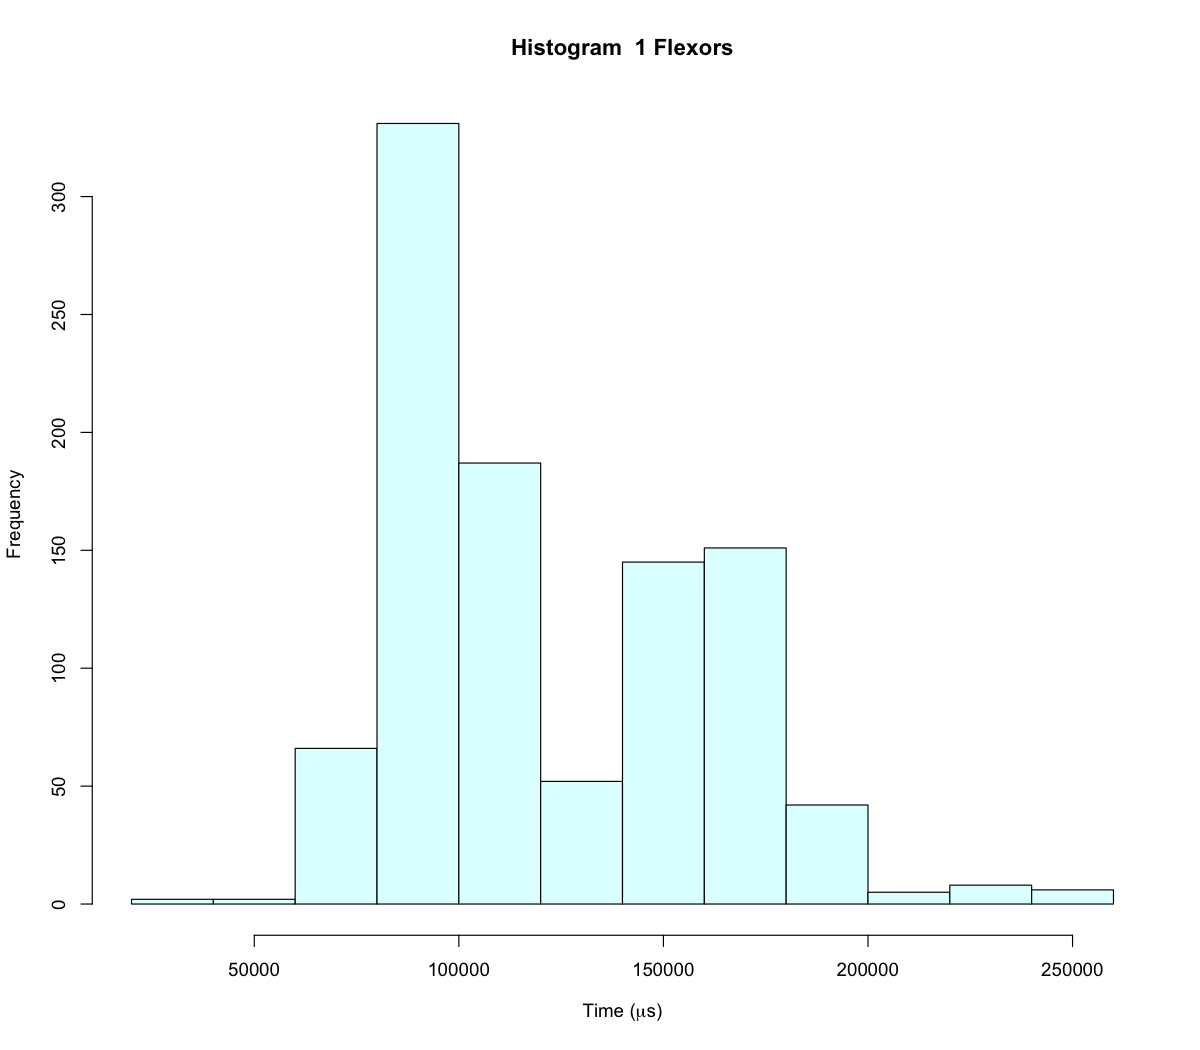
\includegraphics[width=0.5\textwidth]{evaluation/graphics/Droid/Galaxy/HistFlexorsDroidGalaxy.png} 
    \caption[Histogramas de flexores Droid-Galaxy]{Histogramas de flexores  Droid-Galaxy\\Fuente: elaboración propia (2018)} 
    \label{fig:droid-galaxy-hist-flexors}
  \end{center}
\end{figure}

\begin{figure}[H]
  \begin{center} 
   	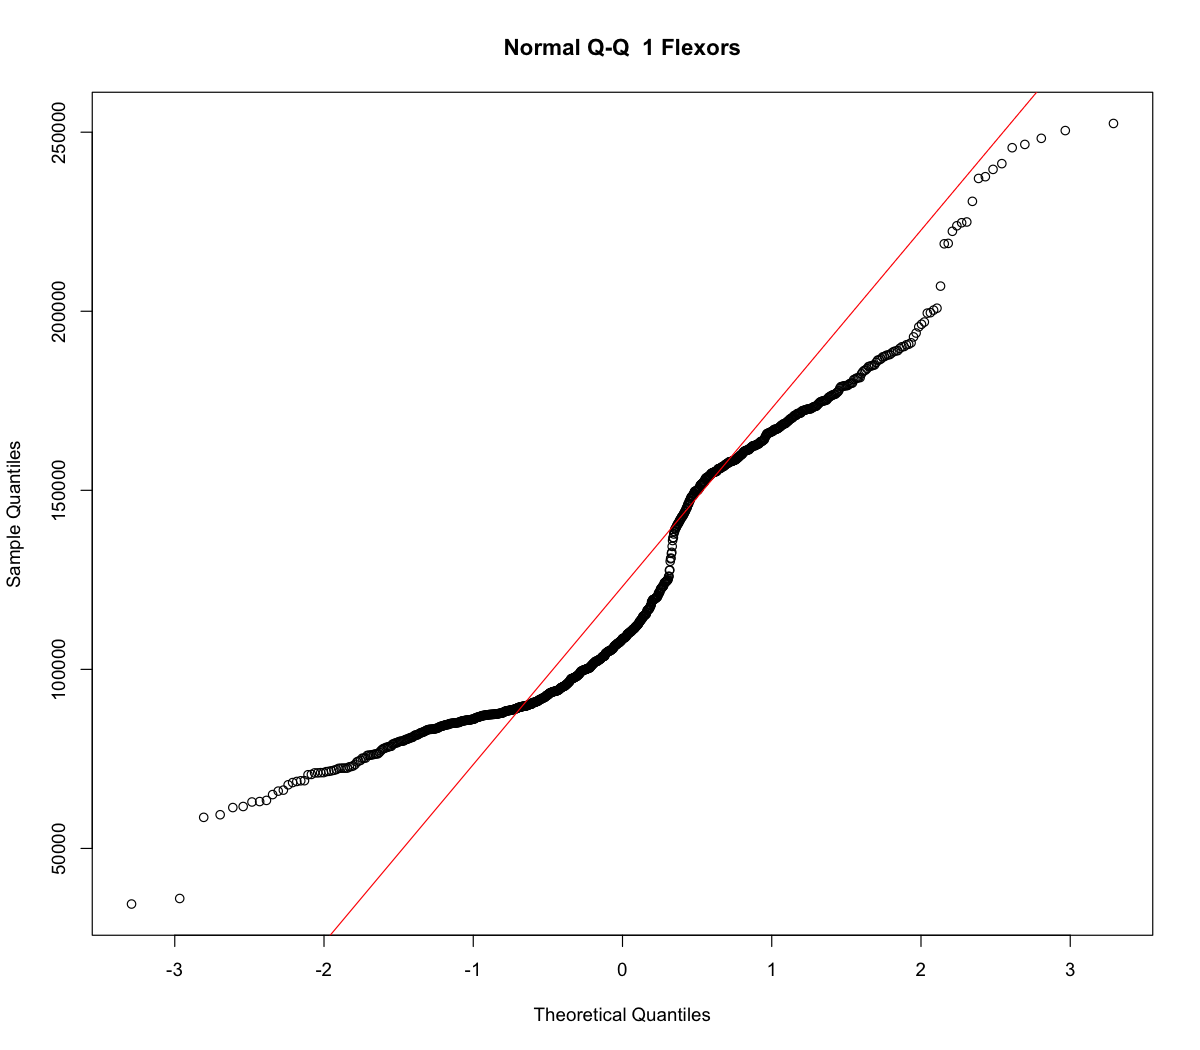
\includegraphics[width=0.5\textwidth]{evaluation/graphics/Droid/Galaxy/NormalQQFlexorsDroidGalaxy.png} 
    \caption[Gráfico QQ de flexores Droid-Galaxy]{Gráficos QQ de flexores Droid-Galaxy\\Fuente: elaboración propia (2018)} 
    \label{fig:droid-galaxy-QQ-flexors}
  \end{center}
\end{figure}

\begin{figure}[H]
  \begin{center} 
   	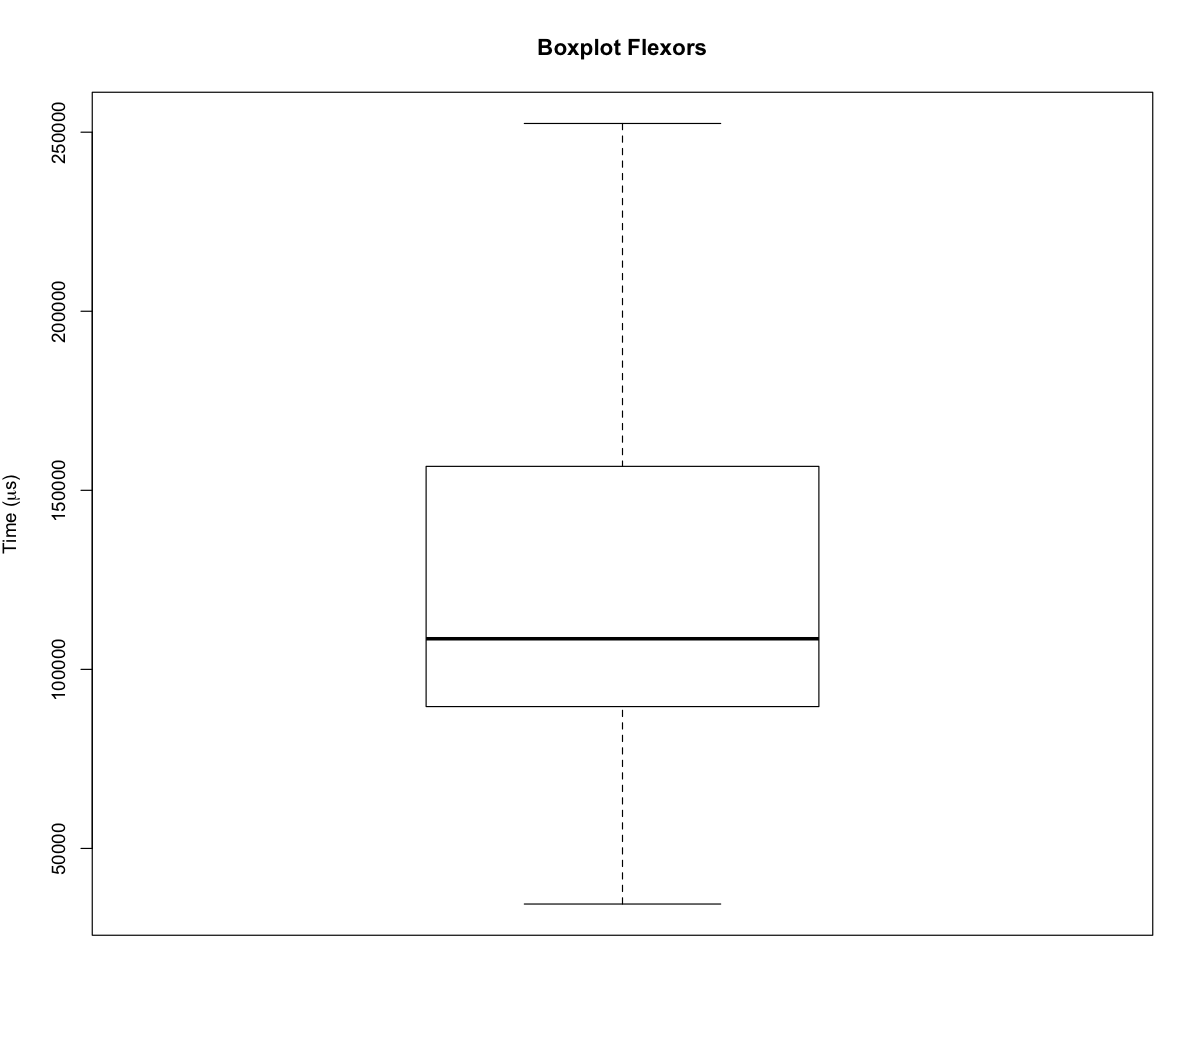
\includegraphics[width=0.5\textwidth]{evaluation/graphics/Droid/Galaxy/BoxplotFlexorsDroidGalaxy.png} 
    \caption[Gráficos de cajas de flexores Droid-Galaxy]{Gráficos de cajas de flexores Droid-Galaxy\\Fuente: elaboración propia (2018)} 
    \label{fig:droid-galaxy-boxplot-flexors}
  \end{center}
\end{figure}





\subsection{Prototipo 4: Xamarin - Galaxy}

\subsubsection{Motores}
% {START} RESUME TABLE ---------------------------------
%\caption[Resumen resultado pruebas motor Xamarin-Galaxy]{Resumen resultado pruebas motor Xamarin-Galaxy \\ Fuente: Elaboración propia (2018)}
%\label{table:motor-xamarin-galaxy}

% Table created by stargazer v.5.2.2 by Marek Hlavac, Harvard University. E-mail: hlavac at fas.harvard.edu
% Date and time: Tue, Jul 03, 2018 - 19:43:49
% Requires LaTeX packages: dcolumn 
\begin{table}[!htbp] \centering 
\caption[Resumen resultado pruebas motor Xamarin-Galaxy]{Resumen resultado pruebas motor Xamarin-Galaxy en $\mu s$ \\ Fuente: Elaboración propia (2018)}
\label{table:motor-xamarin-galaxy}
\begin{tabular}{@{\extracolsep{5pt}} D{.}{.}{-3} D{.}{.}{-3} D{.}{.}{-3} D{.}{.}{-3} D{.}{.}{-3} D{.}{.}{-3} D{.}{.}{-3} D{.}{.}{-3} } 
\\[-1.8ex]\hline 
\hline \\[-1.8ex] 
\multicolumn{1}{c}{Motors} & \multicolumn{1}{c}{Mean} & \multicolumn{1}{c}{Median} & \multicolumn{1}{c}{Min} & \multicolumn{1}{c}{Max} & \multicolumn{1}{c}{Std. Dev.} & \multicolumn{1}{c}{Skewness} & \multicolumn{1}{c}{Kurtosis} \\ 
\hline \\[-1.8ex] 
1 & 299.835 & 268.800 & 231.500 & 512 & 77.214 & 1.376 & 4.065 \\ 
2 & 367.823 & 387.100 & 282 & 600.800 & 59.888 & 0.290 & 2.832 \\ 
3 & 363.318 & 358.200 & 333 & 472.100 & 26.389 & 1.707 & 6.343 \\ 
4 & 491.245 & 506.050 & 380.800 & 785.600 & 78.420 & 0.503 & 3.042 \\ 
5 & 574.120 & 600 & 429.200 & 832.200 & 84.596 & 0.045 & 2.703 \\ 
\hline \\[-1.8ex] 
\end{tabular} 
\end{table} 
% {END} RESUME TABLE ---------------------------------

\begin{figure}
 \begin{center} 
   	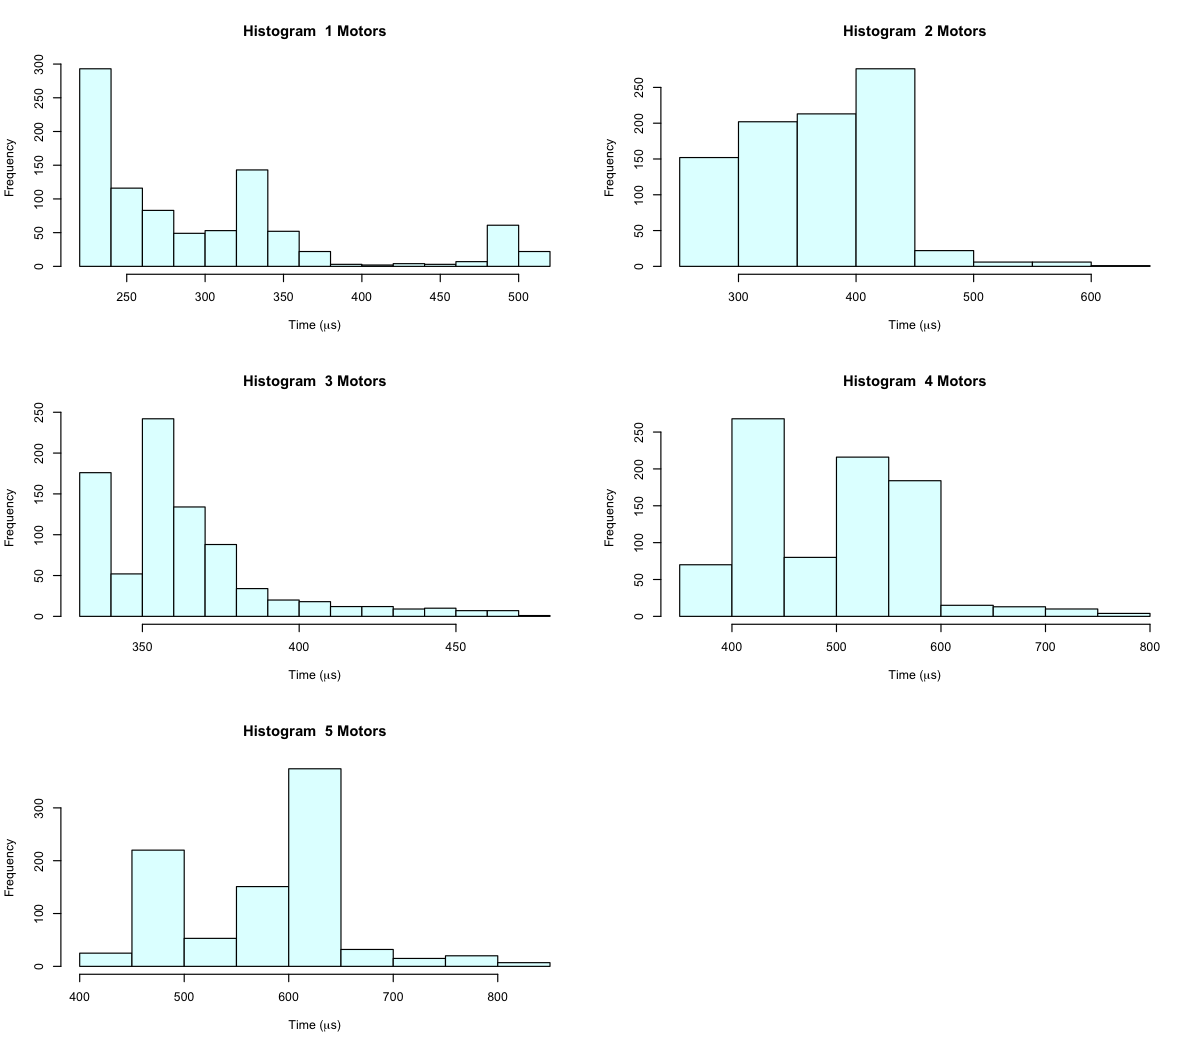
\includegraphics[width=1.0\textwidth]{evaluation/graphics/Xamarin/Galaxy/HistMotorsXamarinGalaxy.png} 
    \caption[Histogramas de motores Xamarin-Galaxy]{Histogramas de motores  Xamarin-Galaxy\\Fuente: elaboración propia (2018)} 
    \label{fig:xamarin-galaxy-hist-motors}
  \end{center}
\end{figure}

\begin{figure}[H]
  \begin{center} 
   	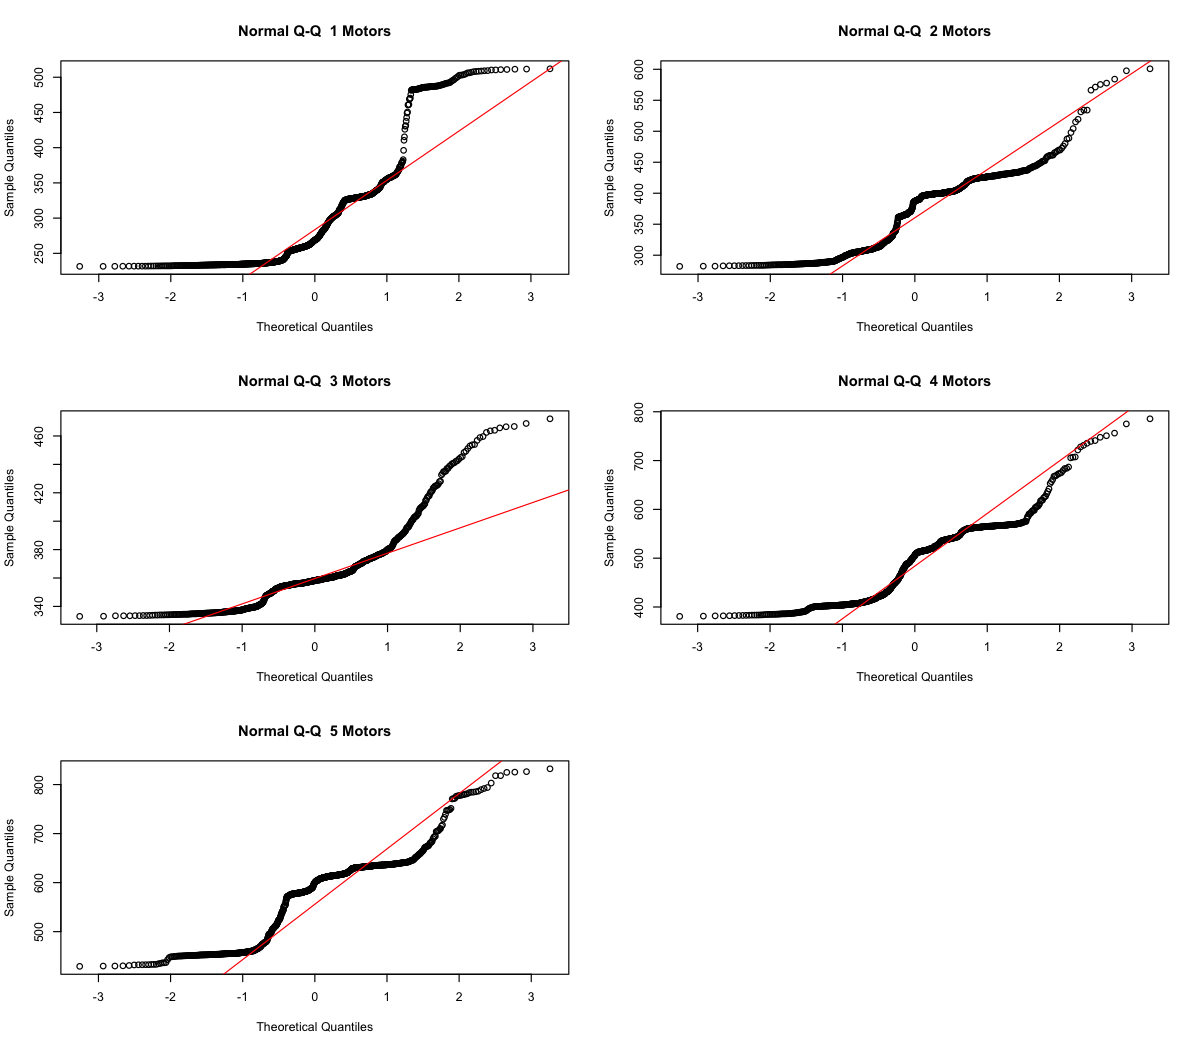
\includegraphics[width=1.0\textwidth]{evaluation/graphics/Xamarin/Galaxy/NormalQQMotorsXamarinGalaxy.png} 
    \caption[Gráfico QQ de motores Xamarin-Galaxy]{Gráficos QQ de motores Xamarin-Galaxy\\Fuente: elaboración propia (2018)} 
    \label{fig:xamarin-galaxy-QQ-motors}
  \end{center}
\end{figure}

\begin{figure}[H]
  \begin{center} 
   	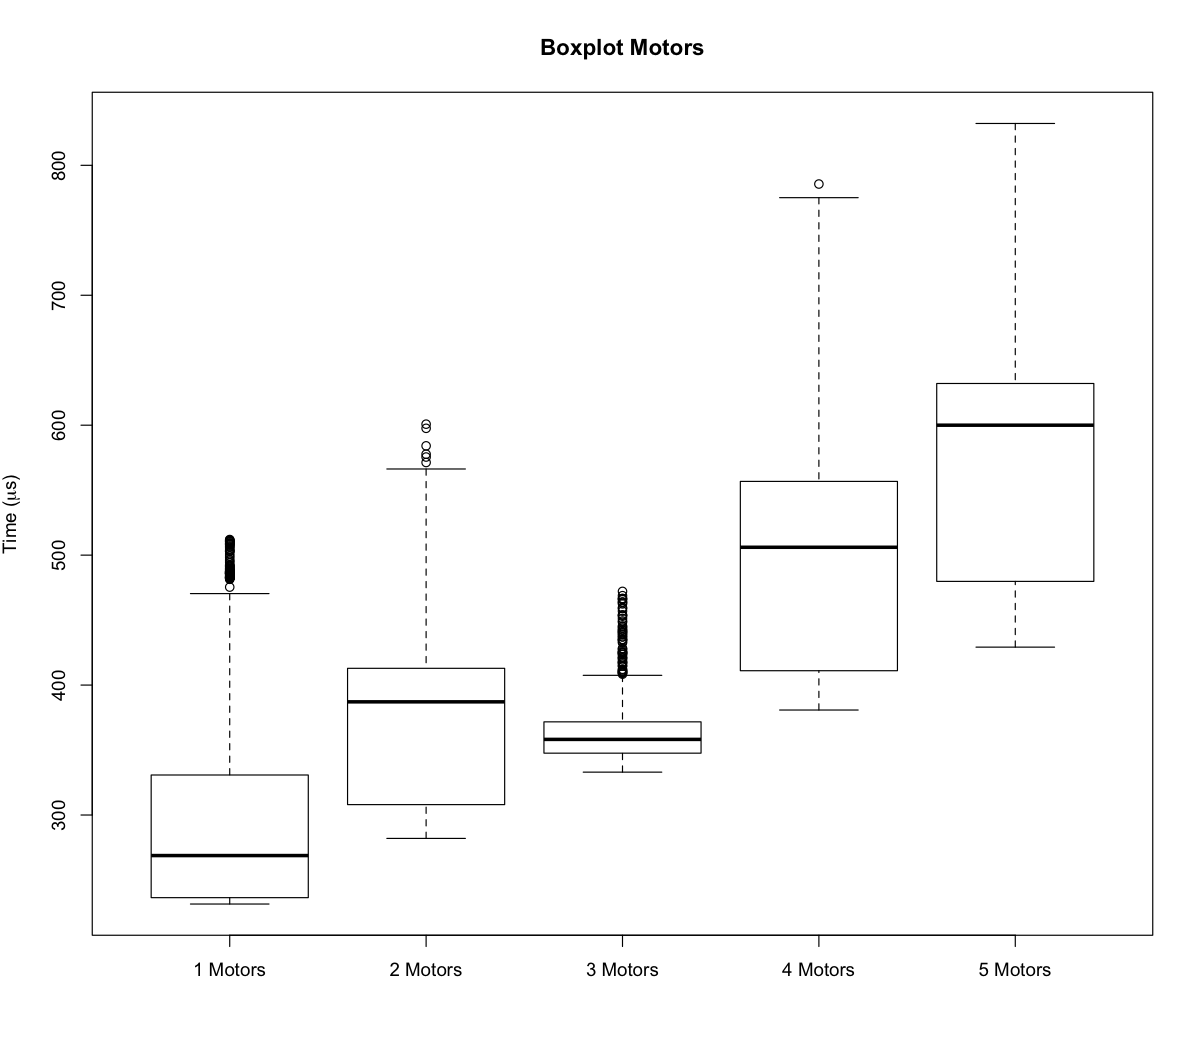
\includegraphics[width=0.8\textwidth]{evaluation/graphics/Xamarin/Galaxy/BoxplotMotorsXamarinGalaxy.png} 
    \caption[Gráficos de cajas de motores Xamarin-Galaxy]{Gráficos de cajas de motores Xamarin-Galaxy\\Fuente: elaboración propia (2018)} 
    \label{fig:xamarin-galaxy-boxplot-motors}
  \end{center}
\end{figure}

\subsubsection{Flexores}
% {START} RESUME TABLE ---------------------------------
%\extracolsep{-11pt}
%\caption[Resumen resultado pruebas flexor Xamarin-Galaxy]{Resumen resultado pruebas flexor Xamarin-Galaxy \\ Fuente: Elaboración propia (2018)}
%\label{table:flexor-xamarin-galaxy}

% Table created by stargazer v.5.2.2 by Marek Hlavac, Harvard University. E-mail: hlavac at fas.harvard.edu
% Date and time: Tue, Jul 03, 2018 - 20:10:45
% Requires LaTeX packages: dcolumn 
\begin{table}[!htbp]
\centering 
\caption[Resumen resultado pruebas flexor Xamarin-Galaxy]{Resumen resultado pruebas flexor Xamarin-Galaxy en $\mu s$\\ Fuente: Elaboración propia (2018)}
\label{table:flexor-xamarin-galaxy}
\begin{tabular}{@{\extracolsep{-11pt}} D{.}{.}{-3} D{.}{.}{-3} D{.}{.}{-3} D{.}{.}{-3} D{.}{.}{-3} D{.}{.}{-3} D{.}{.}{-3} D{.}{.}{-3} } 
\\[-1.8ex]\hline 
\hline \\[-1.8ex] 
\multicolumn{1}{c}{Motors} & \multicolumn{1}{c}{Mean} & \multicolumn{1}{c}{Median} & \multicolumn{1}{c}{Min} & \multicolumn{1}{c}{Max} & \multicolumn{1}{c}{Std. Dev.} & \multicolumn{1}{c}{Skewness} & \multicolumn{1}{c}{Kurtosis} \\ 
\hline \\[-1.8ex] 
1 & 123,483.700 & 109,237.600 & 55,364.200 & 253,747.900 & 39,493.110 & 0.696 & 2.824 \\ 
\hline \\[-1.8ex] 
\end{tabular} 
\end{table} 
% {END} RESUME TABLE ---------------------------------

\begin{figure}
 \begin{center} 
   	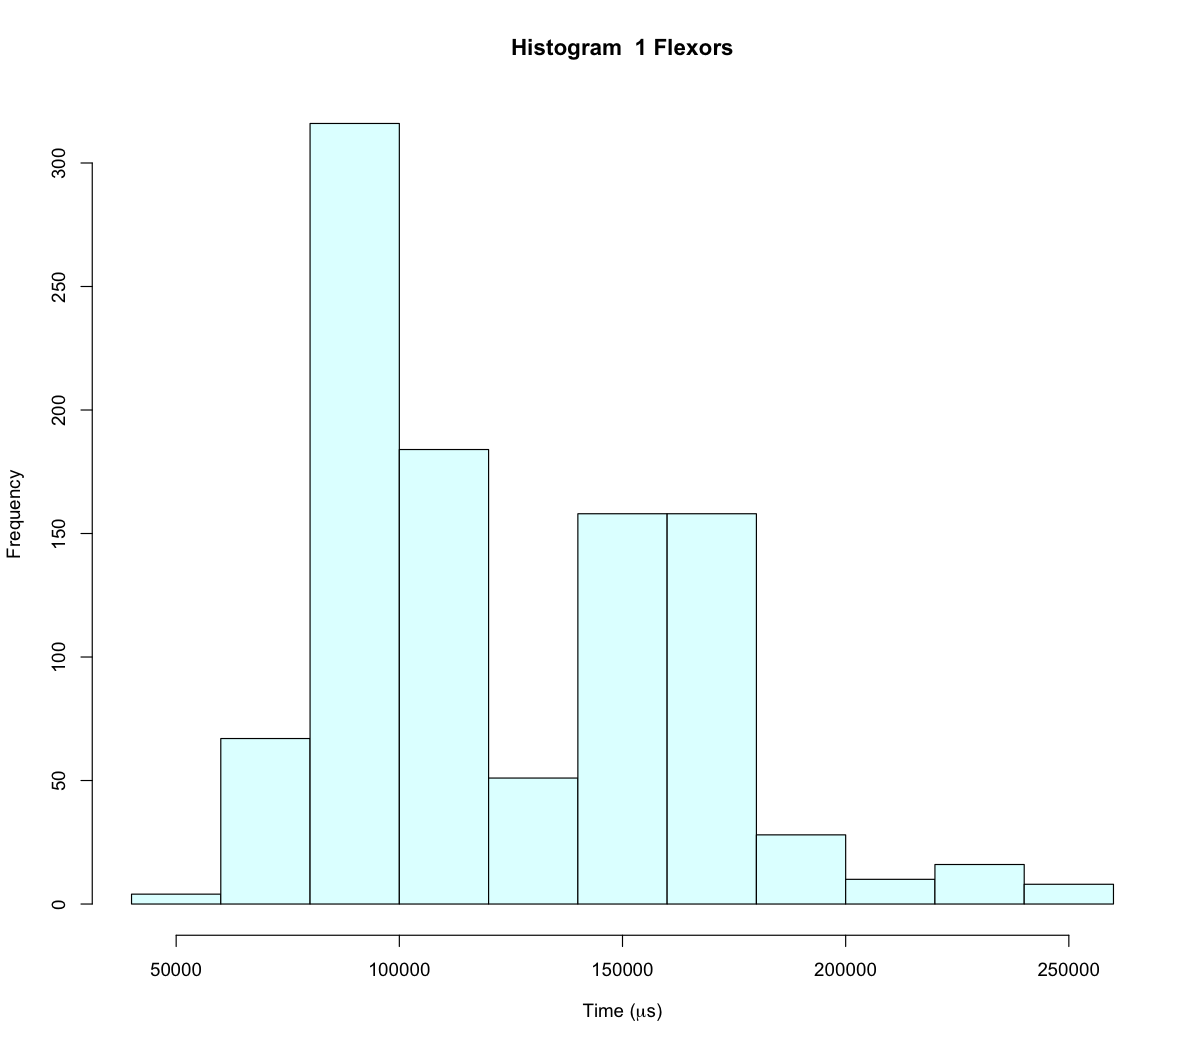
\includegraphics[width=0.5\textwidth]{evaluation/graphics/Xamarin/Galaxy/HistFlexorsXamarinGalaxy.png} 
    \caption[Histogramas de flexores Xamarin-Galaxy]{Histogramas de flexores Xamarin-Galaxy\\Fuente: elaboración propia (2018)} 
    \label{fig:xamarin-galaxy-hist-flexors}
  \end{center}
\end{figure}

\begin{figure}[H]
  \begin{center} 
   	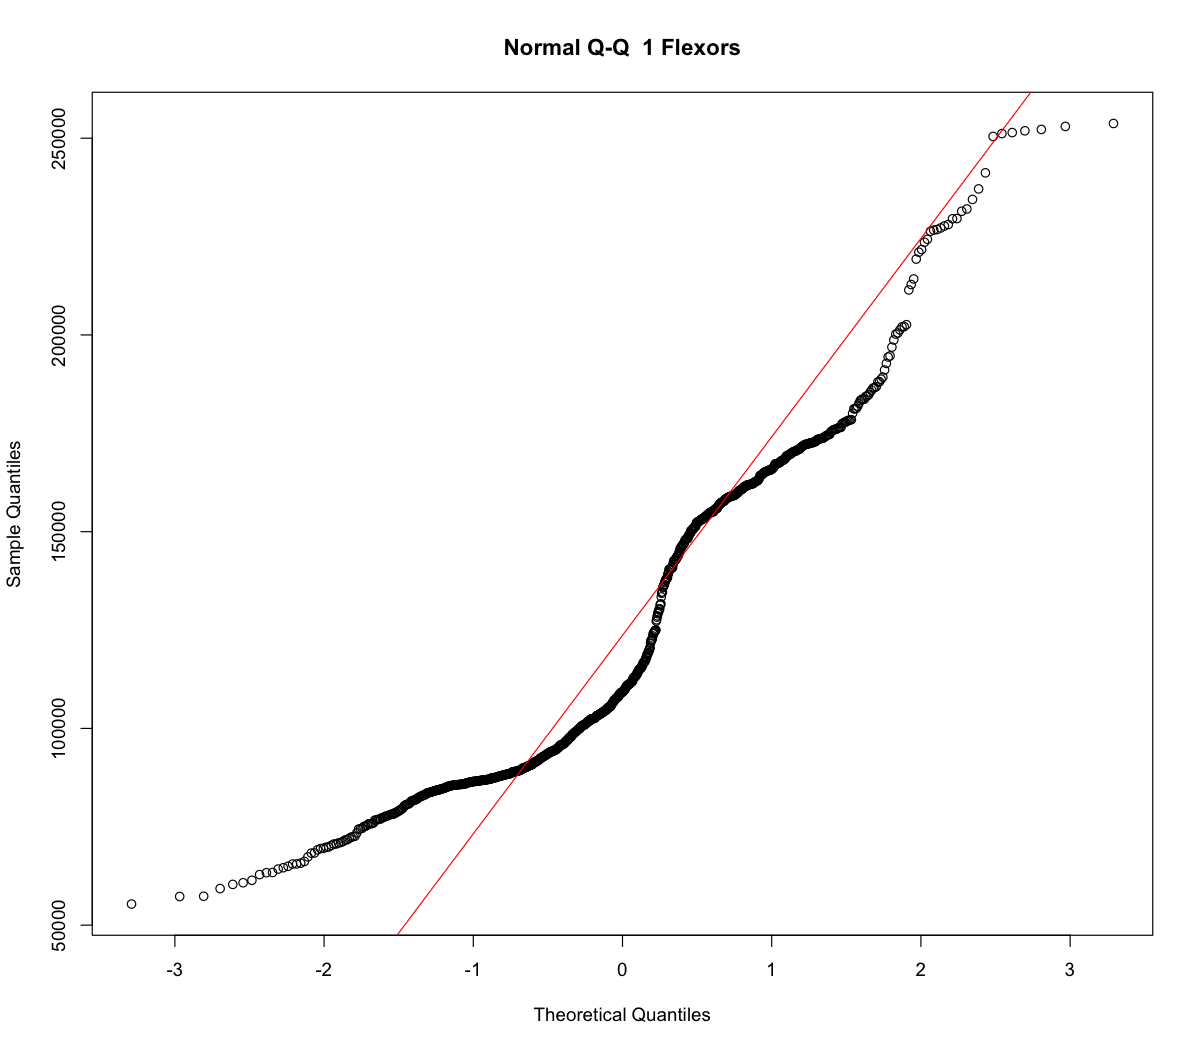
\includegraphics[width=0.5\textwidth]{evaluation/graphics/Xamarin/Galaxy/NormalQQFlexorsXamarinGalaxy.png} 
    \caption[Gráfico QQ de flexores Xamarin-Galaxy]{Gráficos QQ de flexores Xamarin-Galaxy\\Fuente: elaboración propia (2018)} 
    \label{fig:xamarin-galaxy-QQ-flexors}
  \end{center}
\end{figure}

\begin{figure}[H]
  \begin{center} 
   	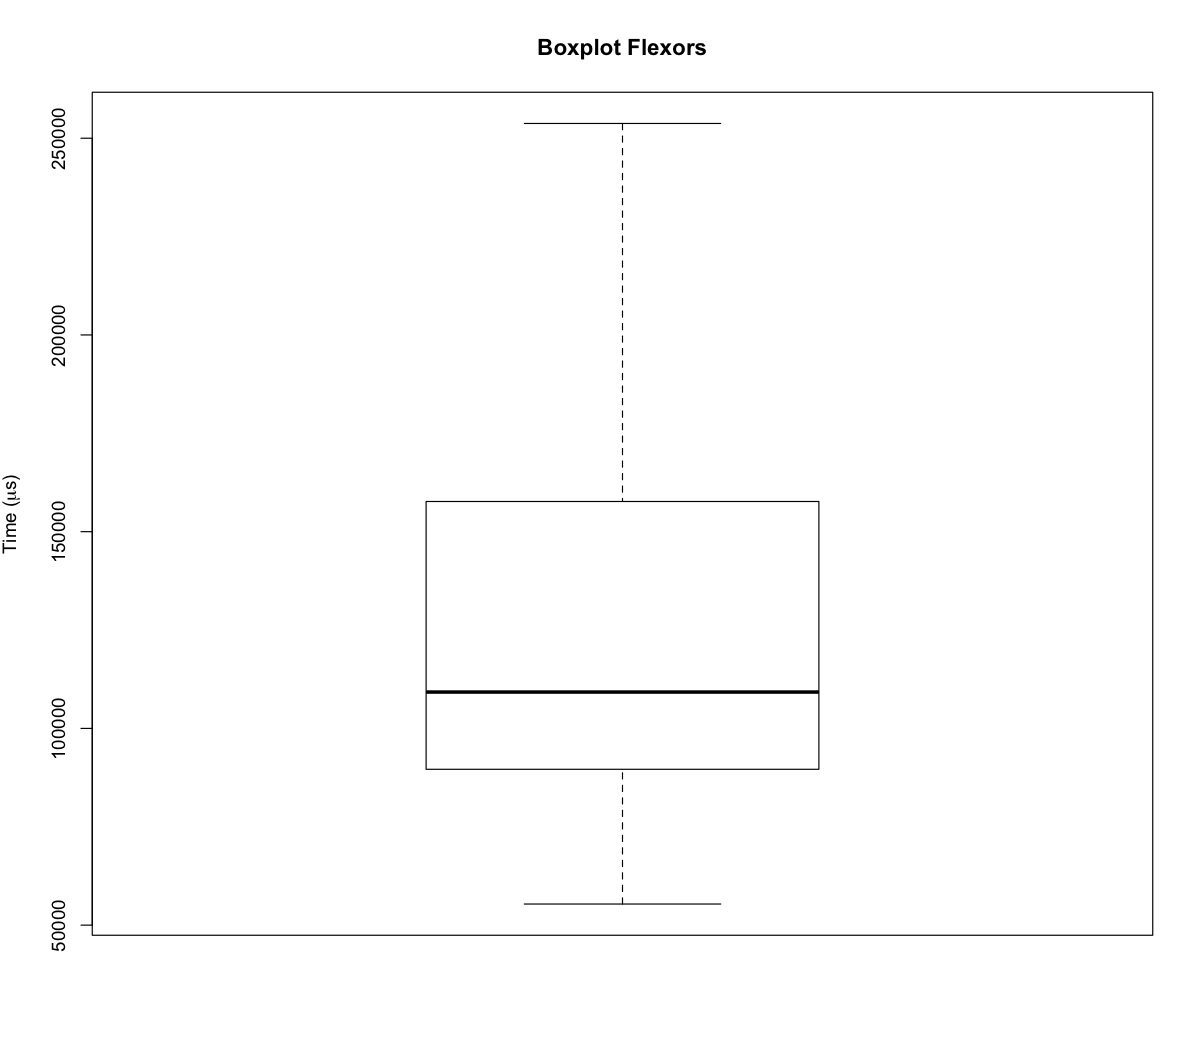
\includegraphics[width=0.5\textwidth]{evaluation/graphics/Xamarin/Galaxy/BoxplotFlexorsXamarinGalaxy.png} 
    \caption[Gráficos de cajas de flexores Xamarin-Galaxy]{Gráficos de cajas de flexores Xamarin-Galaxy\\Fuente: elaboración propia (2018)} 
    \label{fig:xamarin-galaxy-boxplot-flexors}
  \end{center}
\end{figure}



\subsection{Prototipo 3 : Droid - Nexus}

\subsubsection{Motores}
% {START} RESUME TABLE ---------------------------------
%\caption[Resumen resultado pruebas motor Droid-Nexus]{Resumen resultado pruebas motor Droid-Nexus  en $\mu s$\\ Fuente: Elaboración propia (2018)}
%\label{table:motor-droid-nexus} 

% Table created by stargazer v.5.2.2 by Marek Hlavac, Harvard University. E-mail: hlavac at fas.harvard.edu
% Date and time: Tue, Jul 03, 2018 - 19:28:30
% Requires LaTeX packages: dcolumn 
% Table created by stargazer v.5.2.2 by Marek Hlavac, Harvard University. E-mail: hlavac at fas.harvard.edu
% Date and time: Mon, Sep 03, 2018 - 17:49:12
\begin{table}[!htbp] \centering 
\caption[Resumen resultado pruebas motor Droid-Nexus]{Resumen resultado pruebas motor Droid-Nexus  en $\mu s$\\ Fuente: Elaboración propia (2018)}
\label{table:motor-droid-nexus} 
\begin{tabular}{@{\extracolsep{5pt}} cccccccc} 
\\[-1.8ex]\hline 
\hline \\[-1.8ex] 
motors & Mean & Median & Min & Max & Std. Dev. & Skewness & Kurtosis \\ 
\hline \\[-1.8ex] 
$1$ & $187.574$ & $171.979$ & $133.646$ & $335.416$ & $44.577$ & $0.337$ & $1.905$ \\ 
$2$ & $231.251$ & $192.761$ & $168.230$ & $482.136$ & $63.706$ & $0.773$ & $2.835$ \\ 
$3$ & $237.638$ & $220.105$ & $202.812$ & $387.813$ & $44.517$ & $1.965$ & $5.687$ \\ 
$4$ & $262.838$ & $258.646$ & $240.938$ & $391.615$ & $20.442$ & $2.567$ & $13.078$ \\ 
$5$ & $336.917$ & $301.250$ & $276.667$ & $592.553$ & $79.910$ & $1.566$ & $3.872$ \\ 
\hline \\[-1.8ex] 
\end{tabular} 
\end{table} 
% {END} RESUME TABLE ---------------------------------

La Figura \ref{fig:droid-nexus-hist-motors}, muestra los histogramas de las latencias obtenidas al mandar los mensajes de activación y desactivación. Se realizaron pruebas desde uno a cinco motores.

\begin{figure}
 \begin{center} 
   	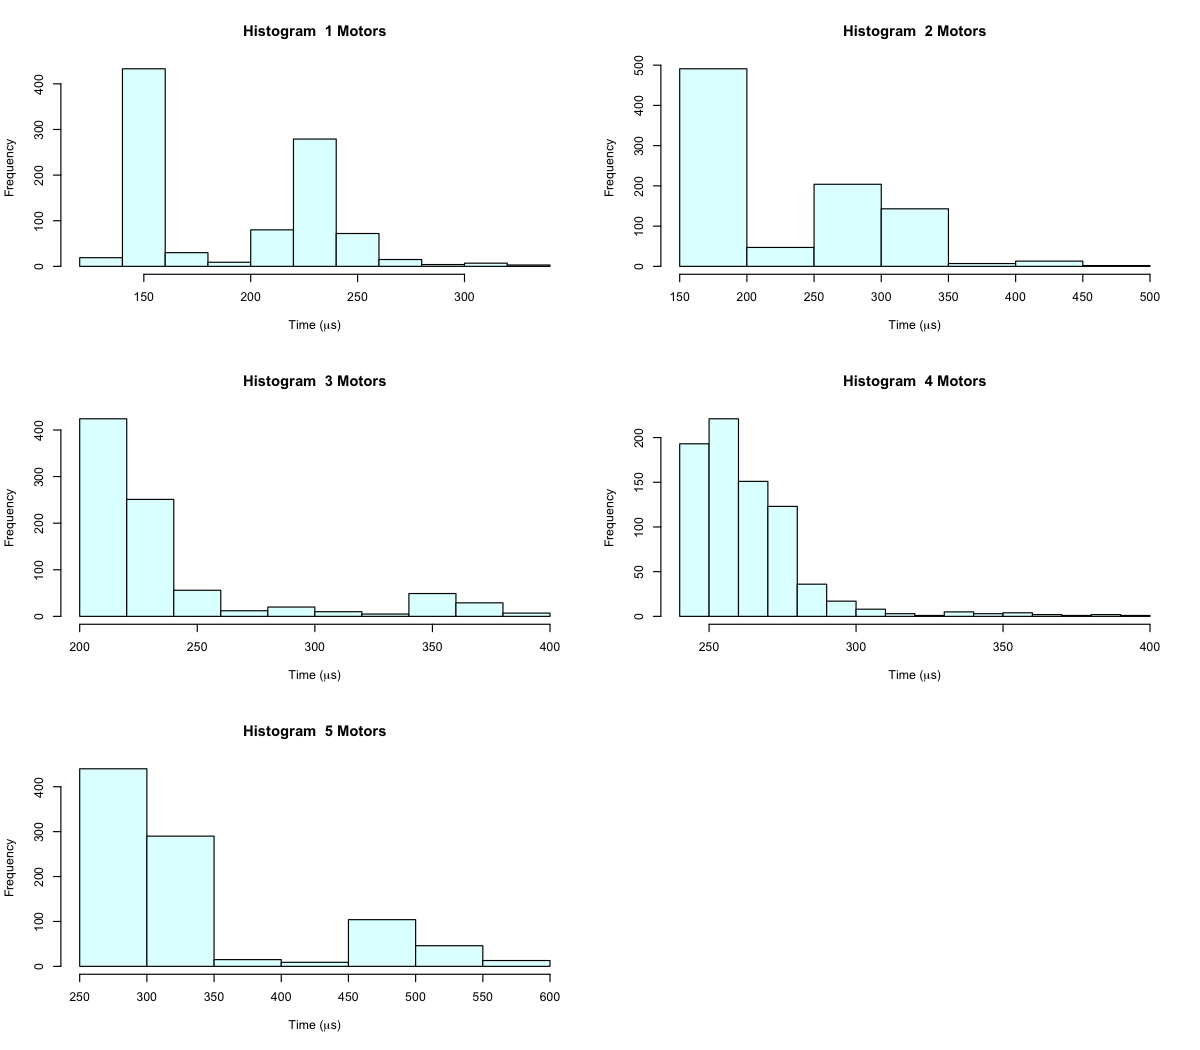
\includegraphics[width=1.0\textwidth]{evaluation/graphics/Droid/Nexus/HistMotorsDroidNexus.png} 
    \caption[Histogramas de motores Droid-Nexus]{Histogramas de motores  Droid-Nexus\\Fuente: elaboración propia (2018)} 
    \label{fig:droid-nexus-hist-motors}
  \end{center}
\end{figure}

\begin{figure}[H]
  \begin{center} 
   	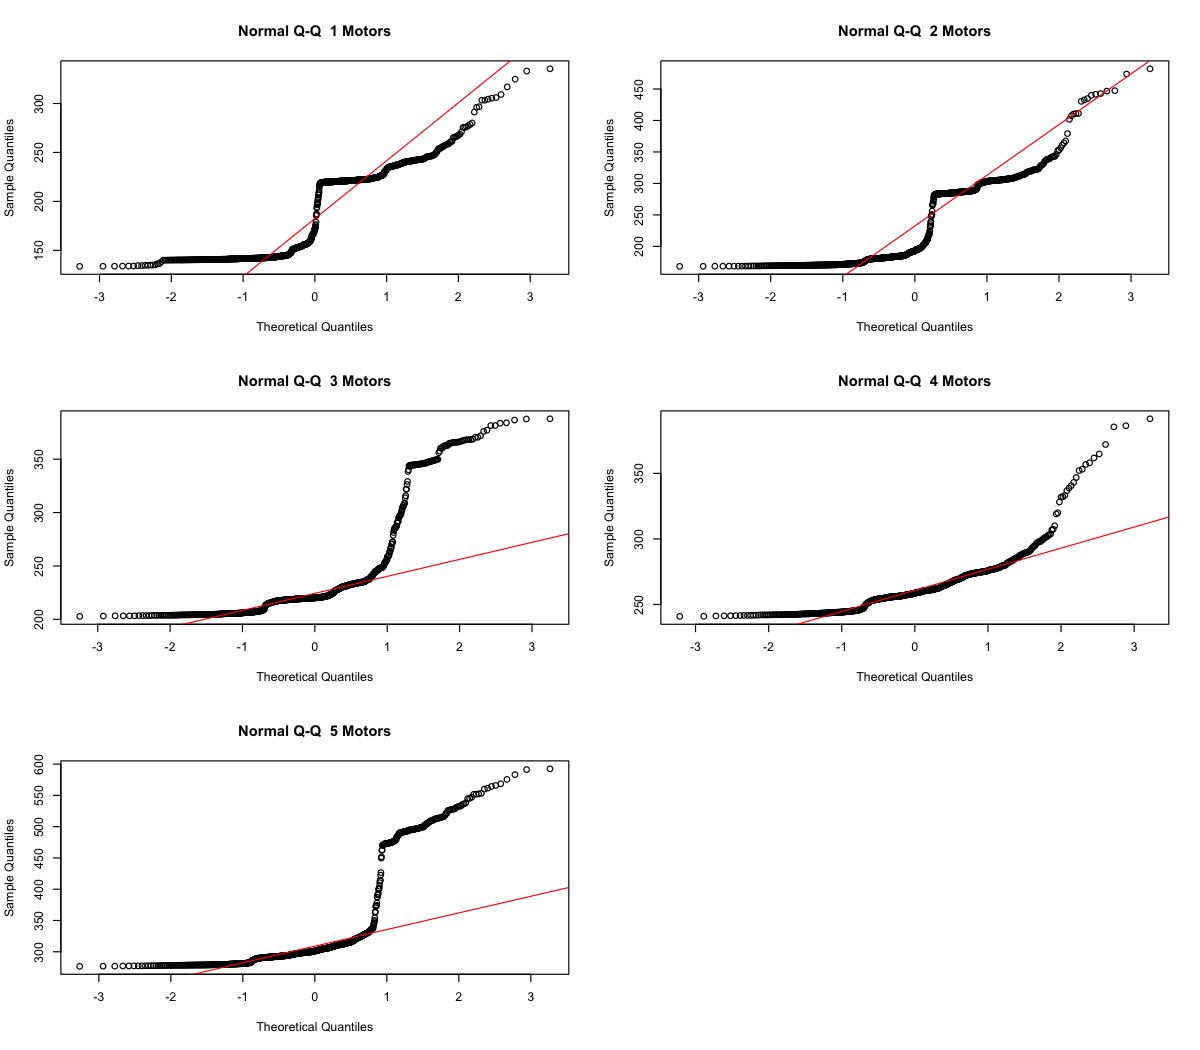
\includegraphics[width=1.0\textwidth]{evaluation/graphics/Droid/Nexus/NormalQQMotorsDroidNexus.png} 
    \caption[Gráfico QQ de motores Droid-Nexus]{Gráficos QQ de motores Droid-Nexus\\Fuente: elaboración propia (2018)} 
    \label{fig:droid-nexus-QQ-motors}
  \end{center}
\end{figure}

\begin{figure}[H]
  \begin{center} 
   	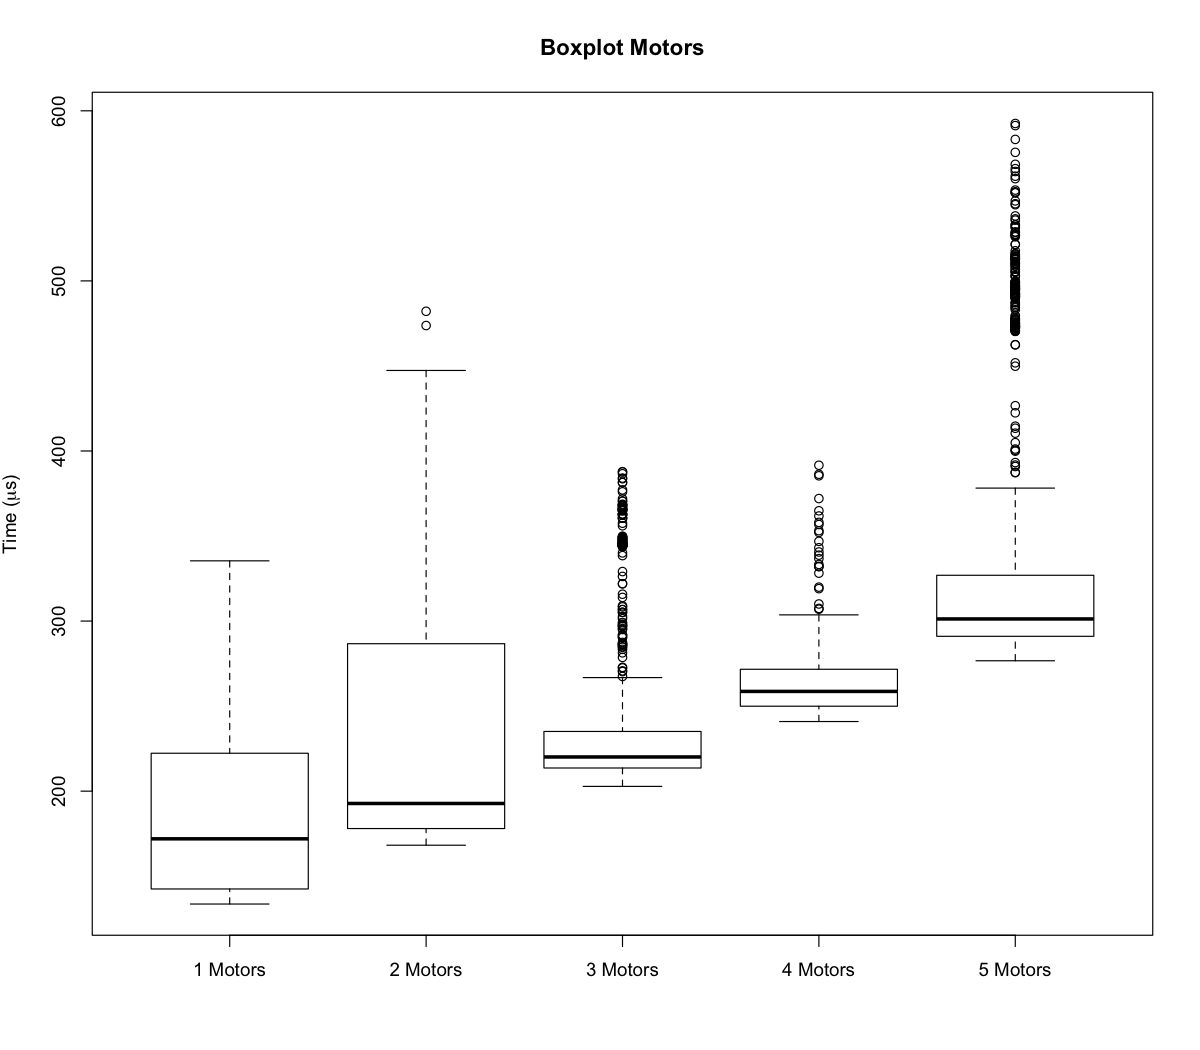
\includegraphics[width=0.8\textwidth]{evaluation/graphics/Droid/Nexus/BoxplotMotorsDroidNexus.png} 
    \caption[Gráficos de cajas de motores Droid-Nexus]{Gráficos de cajas de motores Droid-Nexus\\Fuente: elaboración propia (2018)} 
    \label{fig:droid-nexus-boxplot-motors}
  \end{center}
\end{figure}

\subsubsection{Flexores}
% {START} RESUME TABLE ---------------------------------
%\extracolsep{-11pt}
%\caption[Resumen resultado pruebas flexor Droid-Nexus]{Resumen resultado pruebas flexor Droid-Nexus en $\mu s$\\ Fuente: Elaboración propia (2018)}
%\label{table:flexor-droid-nexus}

% Table created by stargazer v.5.2.2 by Marek Hlavac, Harvard University. E-mail: hlavac at fas.harvard.edu
% Date and time: Mon, Sep 03, 2018 - 17:53:15
\begin{table}[!htbp] \centering 
\caption[Resumen resultado pruebas flexor Droid-Nexus]{Resumen resultado pruebas flexor Droid-Nexus en $\mu s$ \\ Fuente: Elaboración propia (2018)}
\label{table:flexor-droid-nexus}
\begin{tabular}{@{\extracolsep{5pt}} cccccccc} 
\\[-1.8ex]\hline 
\hline \\[-1.8ex] 
flexors & Mean & Median & Min & Max & Std. Dev. & Skewness & Kurtosis \\ 
\hline \\[-1.8ex] 
$1$ & $109,671$ & $114,496$ & $48,099.480$ & $172,982.100$ & $24,155.450$ & $-0.304$ & $2.621$ \\ 
\hline \\[-1.8ex] 
\end{tabular} 
\end{table} 
% {END} RESUME TABLE ---------------------------------

\begin{figure}
 \begin{center} 
   	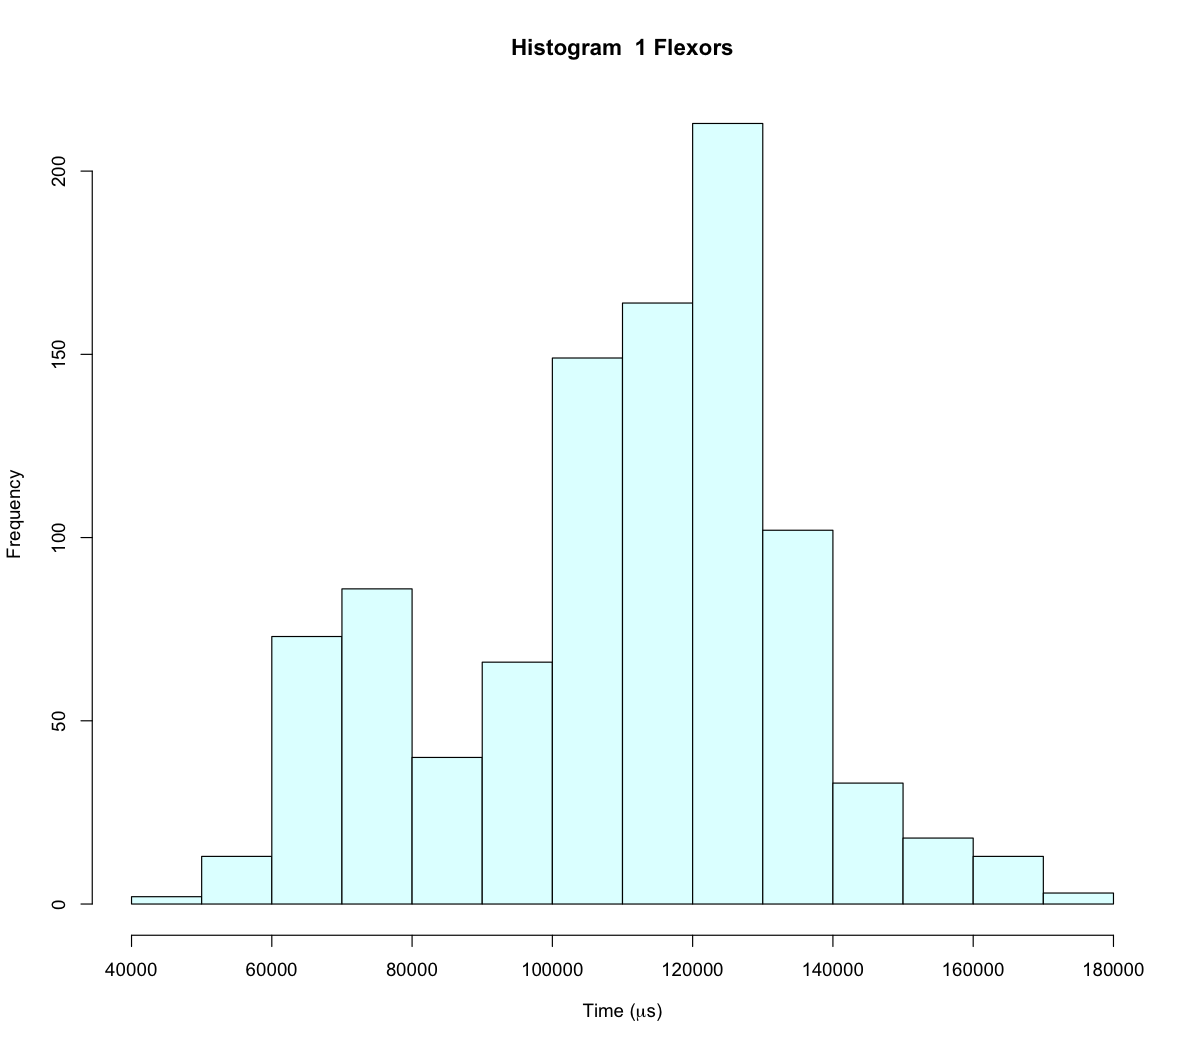
\includegraphics[width=0.5\textwidth]{evaluation/graphics/Droid/Nexus/HistFlexorsDroidNexus.png} 
    \caption[Histogramas de flexores Droid-Nexus]{Histogramas de flexores  Droid-Nexus\\Fuente: elaboración propia (2018)} 
    \label{fig:droid-nexus-hist-flexors}
  \end{center}
\end{figure}

\begin{figure}[H]
  \begin{center} 
   	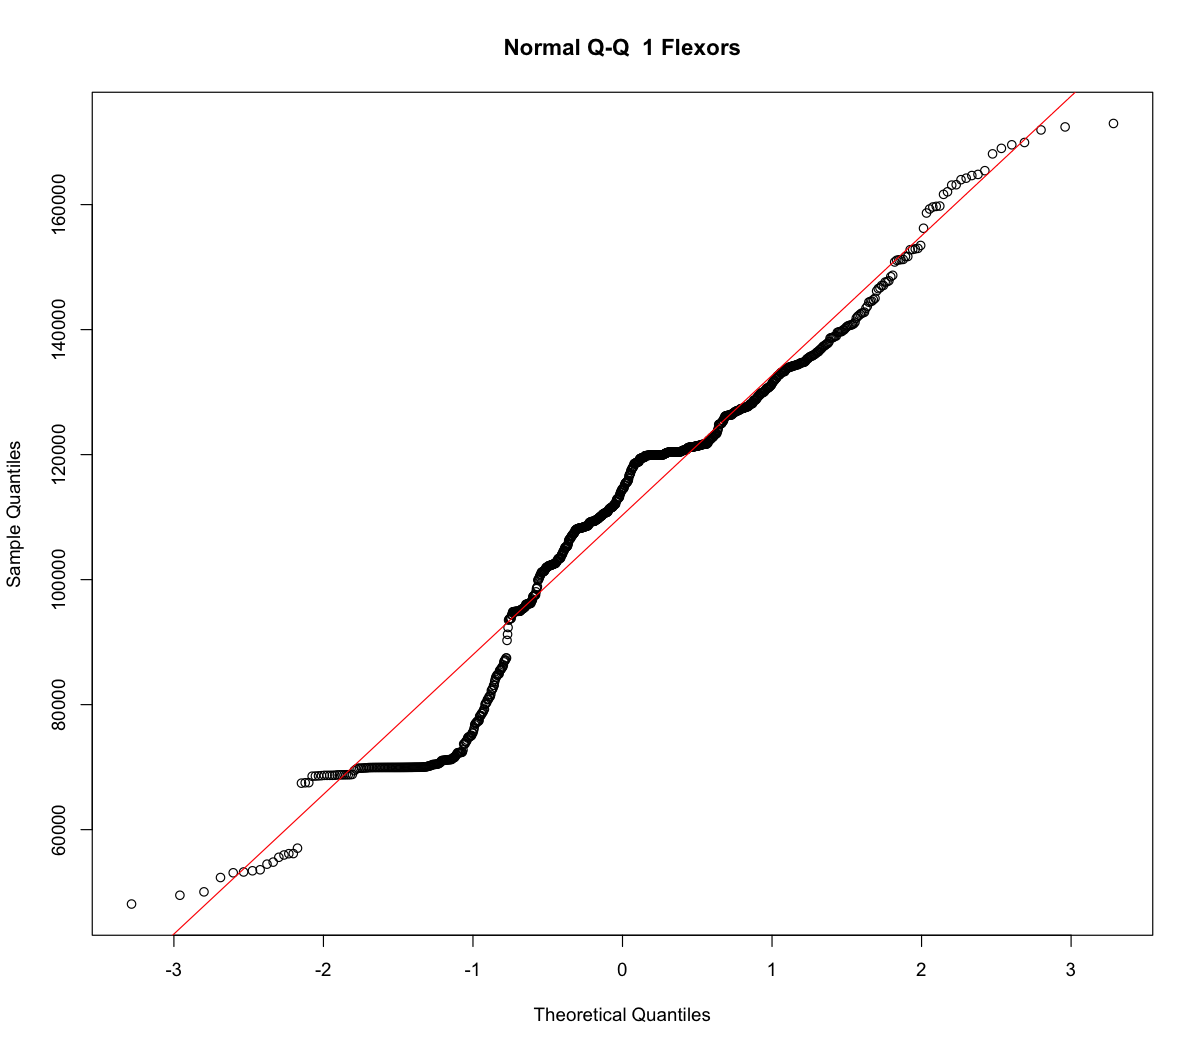
\includegraphics[width=0.5\textwidth]{evaluation/graphics/Droid/Nexus/NormalQQFlexorsDroidNexus.png} 
    \caption[Gráfico QQ de flexores Droid-Nexus]{Gráficos QQ de flexores Droid-Nexus\\Fuente: elaboración propia (2018)} 
    \label{fig:droid-nexus-QQ-flexors}
  \end{center}
\end{figure}

\begin{figure}[H]
  \begin{center} 
   	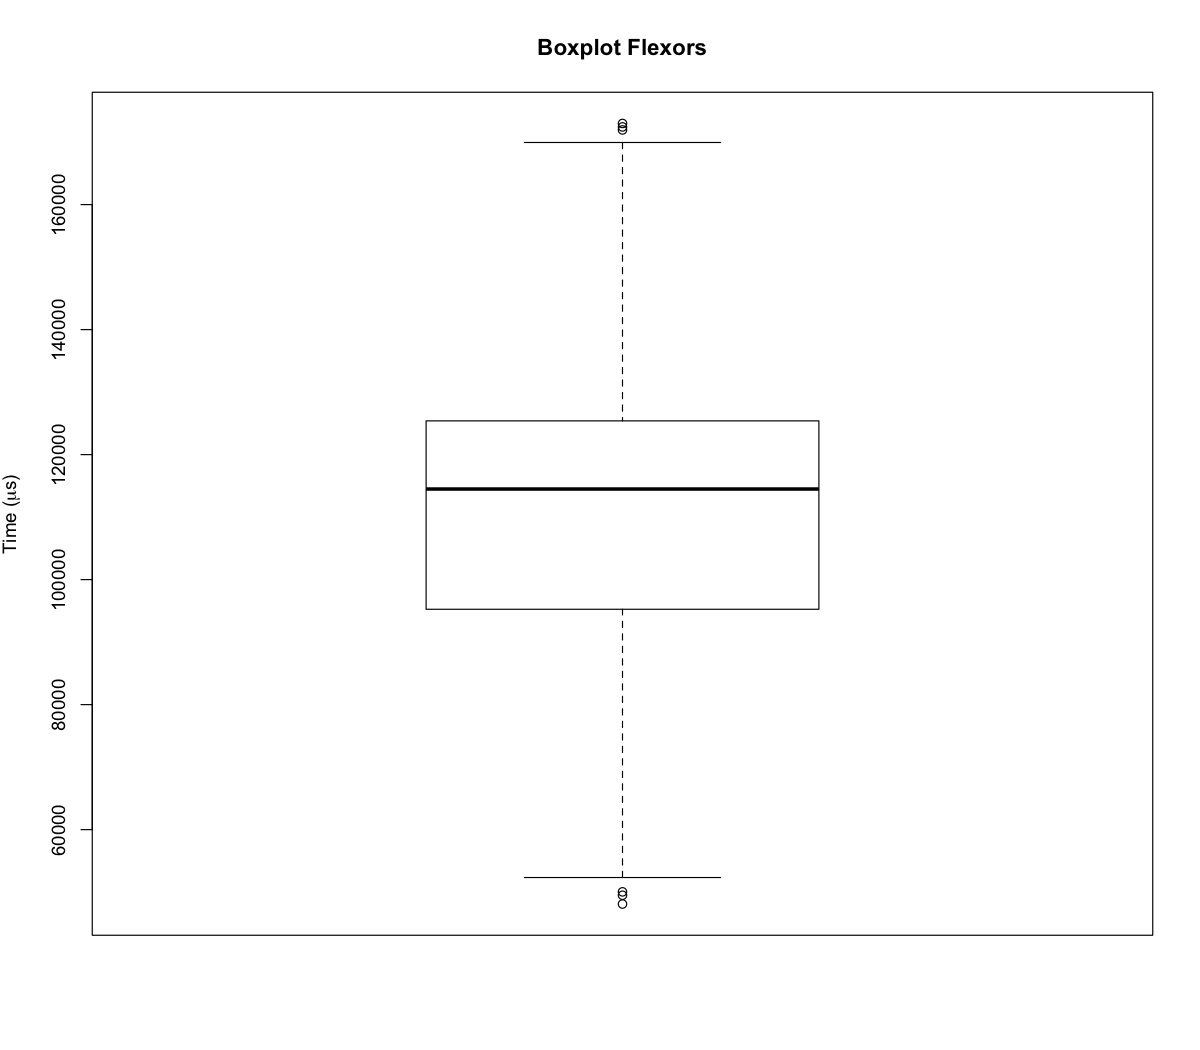
\includegraphics[width=0.5\textwidth]{evaluation/graphics/Droid/Nexus/BoxplotFlexorsDroidNexus.png} 
    \caption[Gráficos de cajas de flexores Droid-Nexus]{Gráficos de cajas de flexores Droid-Nexus\\Fuente: elaboración propia (2018)} 
    \label{fig:droid-nexus-boxplot-flexors}
  \end{center}
\end{figure}

\subsection{Prototipo 4: Xamarin - Nexus}

\subsubsection{Motores}

% {START} RESUME TABLE ---------------------------------
%\caption[Resumen resultado pruebas motor Xamarin-Nexus]{Resumen resultado pruebas motor Xamarin-Nexus  en $\mu s$\\ Fuente: Elaboración propia (2018)}
%\label{table:motor-xamarin-nexus} 

% Table created by stargazer v.5.2.2 by Marek Hlavac, Harvard University. E-mail: hlavac at fas.harvard.edu
% Date and time: Mon, Sep 03, 2018 - 17:56:53
\begin{table}[!htbp] \centering 
\caption[Resumen resultado pruebas motor Xamarin-Nexus]{Resumen resultado pruebas motor Xamarin-Nexus  en $\mu s$\\ Fuente: Elaboración propia (2018)}
\label{table:motor-xamarin-nexus} 
\begin{tabular}{@{\extracolsep{5pt}} cccccccc} 
\\[-1.8ex]\hline 
\hline \\[-1.8ex] 
motors & Mean & Median & Min & Max & Std. Dev. & Skewness & Kurtosis \\ 
\hline \\[-1.8ex] 
$1$ & $206.856$ & $193.600$ & $185.300$ & $288.900$ & $29.516$ & $1.673$ & $4.187$ \\ 
$2$ & $296.004$ & $243.100$ & $225.600$ & $570.200$ & $83.534$ & $0.995$ & $2.558$ \\ 
$3$ & $275.752$ & $275.400$ & $264.100$ & $316.400$ & $8.007$ & $1.078$ & $5.129$ \\ 
$4$ & $309.417$ & $307.950$ & $296.600$ & $333.300$ & $6.822$ & $0.707$ & $3.544$ \\ 
$5$ & $363.526$ & $341.100$ & $328.400$ & $545.300$ & $54.915$ & $2.211$ & $6.235$ \\ 
\hline \\[-1.8ex] 
\end{tabular} 
\end{table} 
% {END} RESUME TABLE ---------------------------------

La Figura \ref{fig:xamarin-nexus-hist-motors}, muestra los histogramas de las latencias obtenidas al mandar los mensajes de activación y desactivación. Se realizaron pruebas desde uno a cinco motores.

\begin{figure}
 \begin{center} 
   	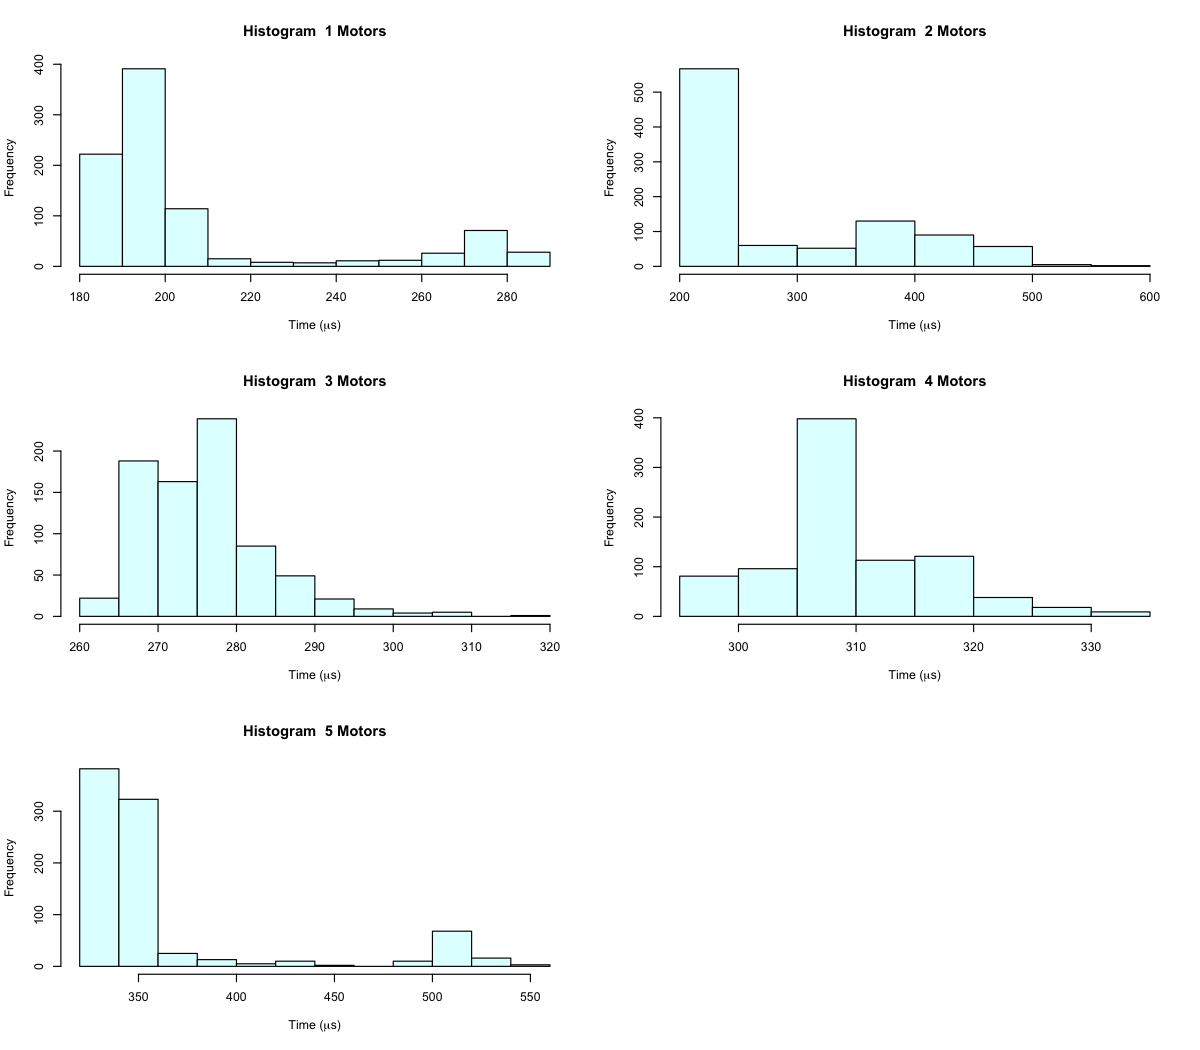
\includegraphics[width=1.0\textwidth]{evaluation/graphics/Xamarin/Nexus/HistMotorsXamarinNexus.png} 
    \caption[Histogramas de motores Xamarin-Nexus]{Histogramas de motores  Xamarin-Nexus\\Fuente: elaboración propia (2018)} 
    \label{fig:xamarin-nexus-hist-motors}
  \end{center}
\end{figure}

\begin{figure}[H]
  \begin{center} 
   	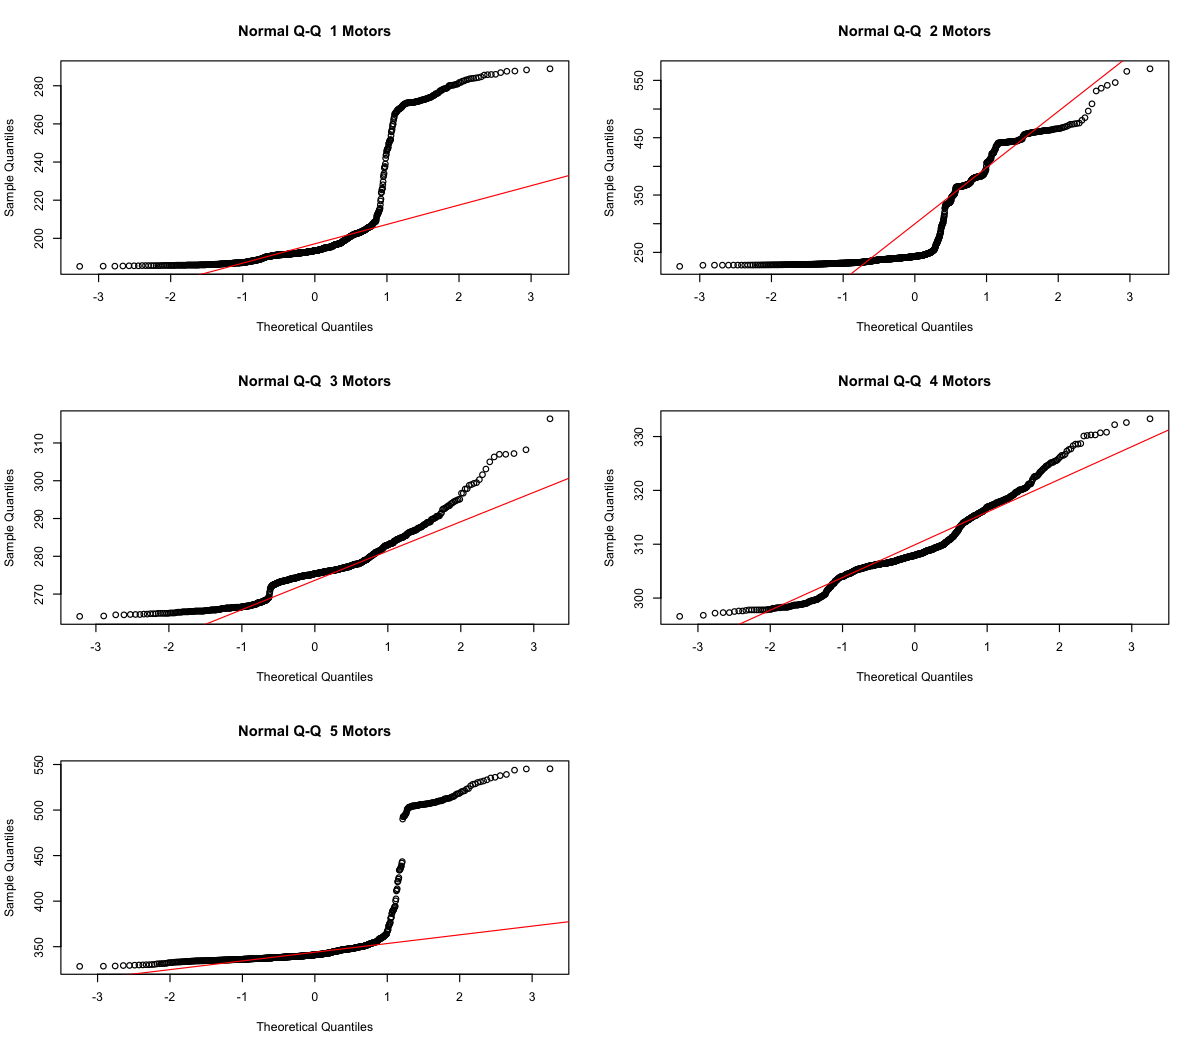
\includegraphics[width=1.0\textwidth]{evaluation/graphics/Xamarin/Nexus/NormalQQMotorsXamarinNexus.png} 
    \caption[Gráfico QQ de motores Xamarin-Nexus]{Gráficos QQ de motores Xamarin-Nexus\\Fuente: elaboración propia (2018)} 
    \label{fig:xamarin-nexus-QQ-motors}
  \end{center}
\end{figure}

\begin{figure}[H]
  \begin{center} 
   	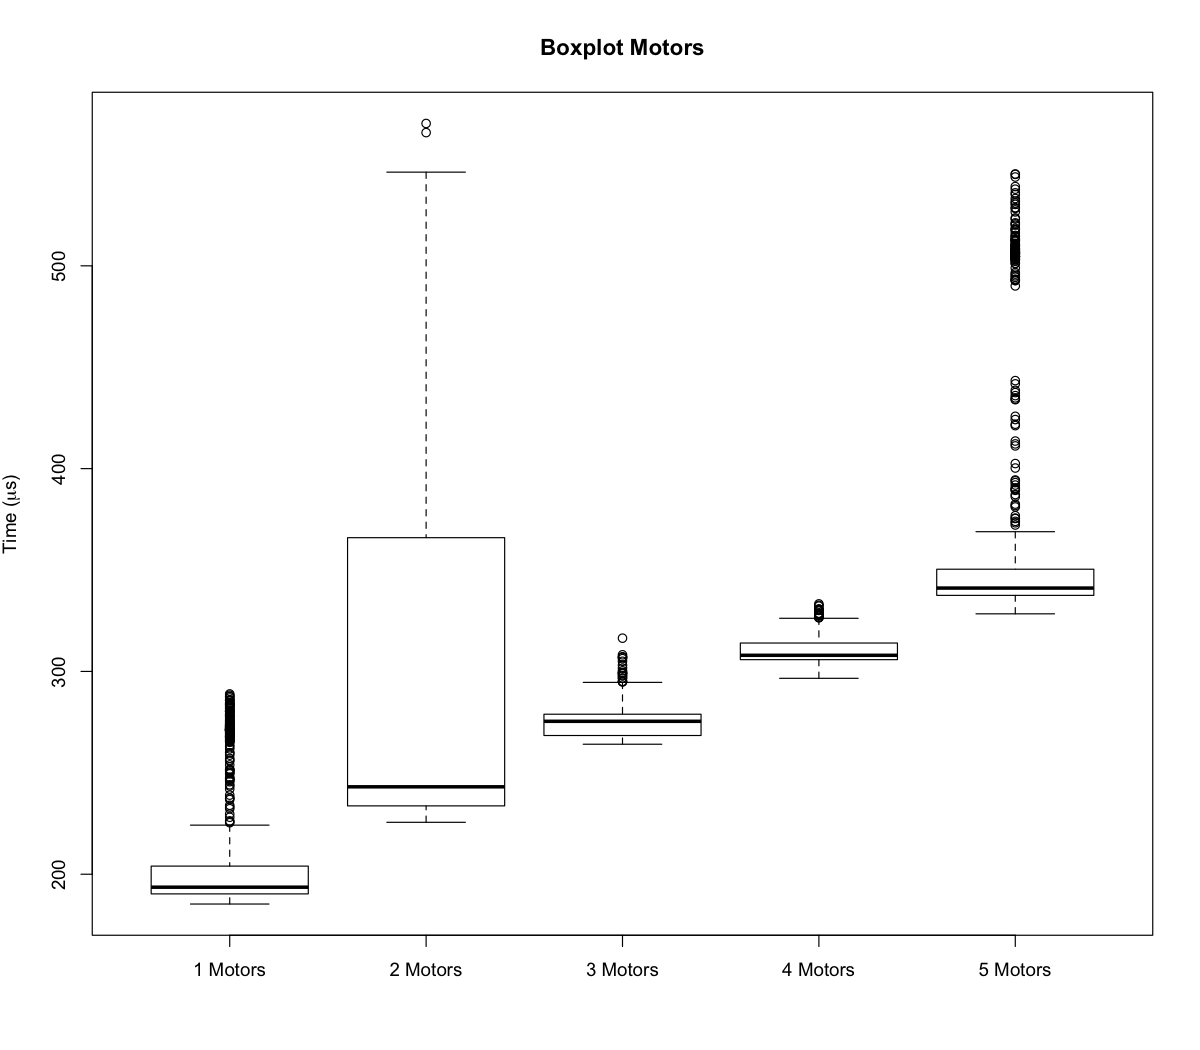
\includegraphics[width=0.8\textwidth]{evaluation/graphics/Xamarin/Nexus/BoxplotMotorsXamarinNexus.png} 
    \caption[Gráficos de cajas de motores Xamarin-Nexus]{Gráficos de cajas de motores Xamarin-Nexus\\Fuente: elaboración propia (2018)} 
    \label{fig:xamarin-nexus-boxplot-motors}
  \end{center}
\end{figure}


\subsubsection{Flexores}

% {START} RESUME TABLE ---------------------------------
%\extracolsep{-11pt}
%\caption[Resumen resultado pruebas flexor Xamarin-Nexus]{Resumen resultado pruebas flexor Xamarin-Nexus en $\mu s$ \\ Fuente: Elaboración propia (2018)}
%\label{table:flexor-xamarin-nexus}

% Table created by stargazer v.5.2.2 by Marek Hlavac, Harvard University. E-mail: hlavac at fas.harvard.edu
% Date and time: Mon, Sep 03, 2018 - 18:04:31
\begin{table}[!htbp] \centering 
\caption[Resumen resultado pruebas flexor Xamarin-Nexus]{Resumen resultado pruebas flexor Xamarin-Nexus en $\mu s$ \\ Fuente: Elaboración propia (2018)}
\label{table:flexor-xamarin-nexus}
\begin{tabular}{@{\extracolsep{5pt}} cccccccc} 
\\[-1.8ex]\hline 
\hline \\[-1.8ex] 
flexors & Mean & Median & Min & Max & Std. Dev. & Skewness & Kurtosis \\ 
\hline \\[-1.8ex] 
$1$ & $109,677$ & $110,958$ & $67,022.400$ & $158,703.500$ & $18,411.270$ & $-0.353$ & $2.914$ \\ 
\hline \\[-1.8ex] 
\end{tabular} 
\end{table} 
% {END} RESUME TABLE ---------------------------------

\begin{figure}
 \begin{center} 
   	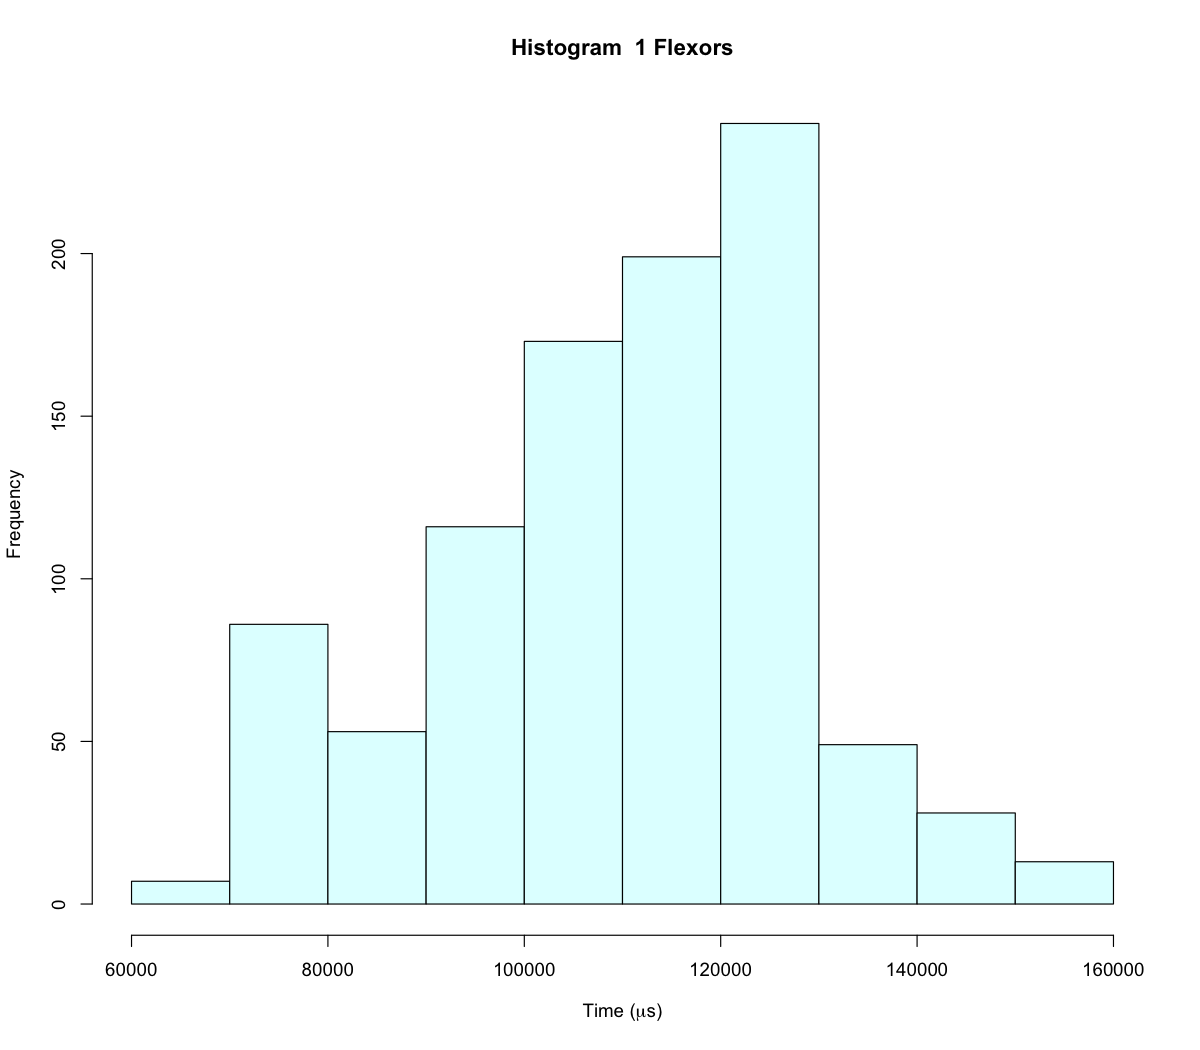
\includegraphics[width=0.5\textwidth]{evaluation/graphics/Xamarin/Nexus/HistFlexorsXamarinNexus.png} 
    \caption[Histogramas de flexores Xamarin-Nexus]{Histogramas de flexores  Xamarin-Nexus\\Fuente: elaboración propia (2018)} 
    \label{fig:xamarin-nexus-hist-flexors}
  \end{center}
\end{figure}

\begin{figure}[H]
  \begin{center} 
   	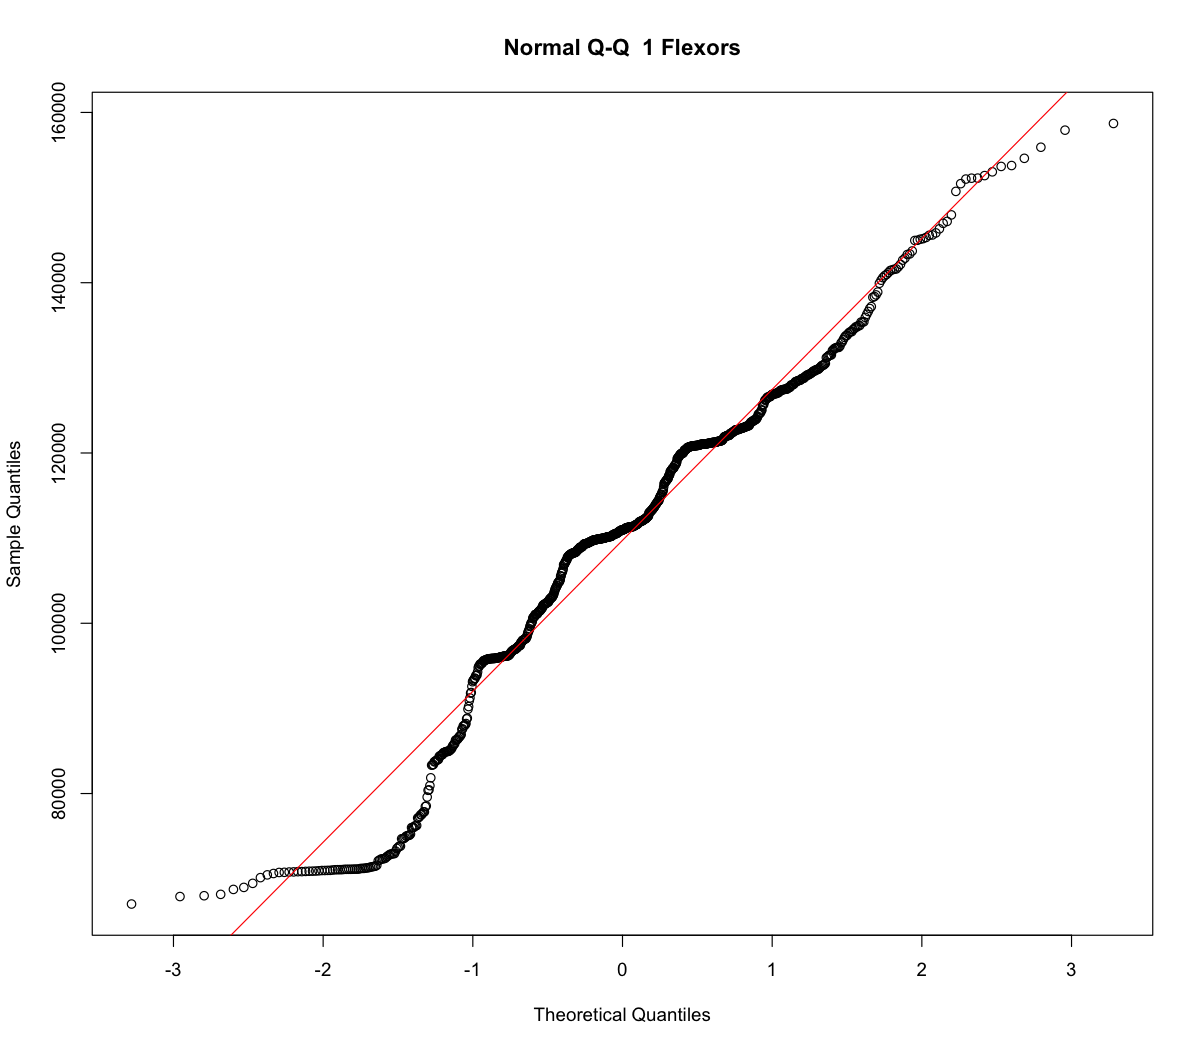
\includegraphics[width=0.5\textwidth]{evaluation/graphics/Xamarin/Nexus/NormalQQFlexorsXamarinNexus.png} 
    \caption[Gráfico QQ de flexores Xamarin-Nexus]{Gráficos QQ de flexores Xamarin-Nexus\\Fuente: elaboración propia (2018)} 
    \label{fig:xamarin-nexus-QQ-flexors}
  \end{center}
\end{figure}

\begin{figure}[H]
  \begin{center} 
   	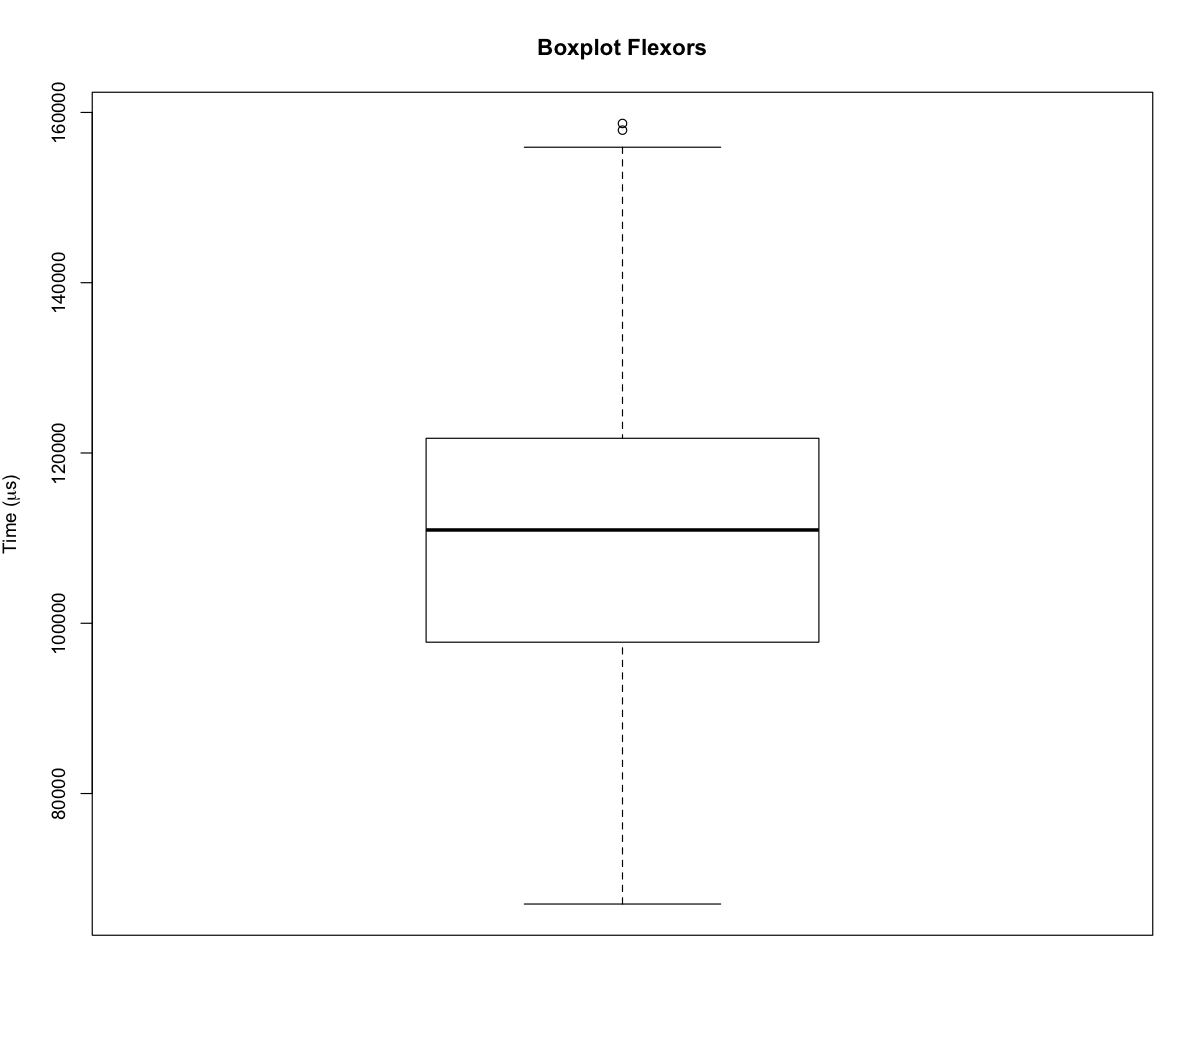
\includegraphics[width=0.5\textwidth]{evaluation/graphics/Xamarin/Nexus/BoxplotFlexorsXamarinNexus.png} 
    \caption[Gráficos de cajas de flexores Xamarin-Nexus]{Gráficos de cajas de flexores Xamarin-Nexus\\Fuente: elaboración propia (2018)} 
    \label{fig:xamarin-nexus-boxplot-flexors}
  \end{center}
\end{figure}
